\documentclass[]{tufte-book}

% ams
\usepackage{amssymb,amsmath}

\usepackage{ifxetex,ifluatex}
\usepackage{fixltx2e} % provides \textsubscript
\ifnum 0\ifxetex 1\fi\ifluatex 1\fi=0 % if pdftex
  \usepackage[T1]{fontenc}
  \usepackage[utf8]{inputenc}
\else % if luatex or xelatex
  \makeatletter
  \@ifpackageloaded{fontspec}{}{\usepackage{fontspec}}
  \makeatother
  \defaultfontfeatures{Ligatures=TeX,Scale=MatchLowercase}
  \makeatletter
  \@ifpackageloaded{soul}{
     \renewcommand\allcapsspacing[1]{{\addfontfeature{LetterSpace=15}#1}}
     \renewcommand\smallcapsspacing[1]{{\addfontfeature{LetterSpace=10}#1}}
   }{}
  \makeatother

\fi

% graphix
\usepackage{graphicx}
\setkeys{Gin}{width=\linewidth,totalheight=\textheight,keepaspectratio}

% booktabs
\usepackage{booktabs}

% url
\usepackage{url}

% hyperref
\usepackage{hyperref}

% units.
\usepackage{units}


\setcounter{secnumdepth}{-1}

% citations

% pandoc syntax highlighting
\usepackage{color}
\usepackage{fancyvrb}
\newcommand{\VerbBar}{|}
\newcommand{\VERB}{\Verb[commandchars=\\\{\}]}
\DefineVerbatimEnvironment{Highlighting}{Verbatim}{commandchars=\\\{\}}
% Add ',fontsize=\small' for more characters per line
\newenvironment{Shaded}{}{}
\newcommand{\AlertTok}[1]{\textcolor[rgb]{1.00,0.00,0.00}{\textbf{#1}}}
\newcommand{\AnnotationTok}[1]{\textcolor[rgb]{0.38,0.63,0.69}{\textbf{\textit{#1}}}}
\newcommand{\AttributeTok}[1]{\textcolor[rgb]{0.49,0.56,0.16}{#1}}
\newcommand{\BaseNTok}[1]{\textcolor[rgb]{0.25,0.63,0.44}{#1}}
\newcommand{\BuiltInTok}[1]{#1}
\newcommand{\CharTok}[1]{\textcolor[rgb]{0.25,0.44,0.63}{#1}}
\newcommand{\CommentTok}[1]{\textcolor[rgb]{0.38,0.63,0.69}{\textit{#1}}}
\newcommand{\CommentVarTok}[1]{\textcolor[rgb]{0.38,0.63,0.69}{\textbf{\textit{#1}}}}
\newcommand{\ConstantTok}[1]{\textcolor[rgb]{0.53,0.00,0.00}{#1}}
\newcommand{\ControlFlowTok}[1]{\textcolor[rgb]{0.00,0.44,0.13}{\textbf{#1}}}
\newcommand{\DataTypeTok}[1]{\textcolor[rgb]{0.56,0.13,0.00}{#1}}
\newcommand{\DecValTok}[1]{\textcolor[rgb]{0.25,0.63,0.44}{#1}}
\newcommand{\DocumentationTok}[1]{\textcolor[rgb]{0.73,0.13,0.13}{\textit{#1}}}
\newcommand{\ErrorTok}[1]{\textcolor[rgb]{1.00,0.00,0.00}{\textbf{#1}}}
\newcommand{\ExtensionTok}[1]{#1}
\newcommand{\FloatTok}[1]{\textcolor[rgb]{0.25,0.63,0.44}{#1}}
\newcommand{\FunctionTok}[1]{\textcolor[rgb]{0.02,0.16,0.49}{#1}}
\newcommand{\ImportTok}[1]{#1}
\newcommand{\InformationTok}[1]{\textcolor[rgb]{0.38,0.63,0.69}{\textbf{\textit{#1}}}}
\newcommand{\KeywordTok}[1]{\textcolor[rgb]{0.00,0.44,0.13}{\textbf{#1}}}
\newcommand{\NormalTok}[1]{#1}
\newcommand{\OperatorTok}[1]{\textcolor[rgb]{0.40,0.40,0.40}{#1}}
\newcommand{\OtherTok}[1]{\textcolor[rgb]{0.00,0.44,0.13}{#1}}
\newcommand{\PreprocessorTok}[1]{\textcolor[rgb]{0.74,0.48,0.00}{#1}}
\newcommand{\RegionMarkerTok}[1]{#1}
\newcommand{\SpecialCharTok}[1]{\textcolor[rgb]{0.25,0.44,0.63}{#1}}
\newcommand{\SpecialStringTok}[1]{\textcolor[rgb]{0.73,0.40,0.53}{#1}}
\newcommand{\StringTok}[1]{\textcolor[rgb]{0.25,0.44,0.63}{#1}}
\newcommand{\VariableTok}[1]{\textcolor[rgb]{0.10,0.09,0.49}{#1}}
\newcommand{\VerbatimStringTok}[1]{\textcolor[rgb]{0.25,0.44,0.63}{#1}}
\newcommand{\WarningTok}[1]{\textcolor[rgb]{0.38,0.63,0.69}{\textbf{\textit{#1}}}}

% longtable
\usepackage{longtable,booktabs}

% multiplecol
\usepackage{multicol}

% strikeout
\usepackage[normalem]{ulem}

% morefloats
\usepackage{morefloats}


% tightlist macro required by pandoc >= 1.14
\providecommand{\tightlist}{%
  \setlength{\itemsep}{0pt}\setlength{\parskip}{0pt}}

% title / author / date
\title{Mathematical Statistics I}
\date{June 16, 2019}


\begin{document}

\maketitle




\hypertarget{section}{%
\chapter{}\label{section}}

\hypertarget{prabability-theory}{%
\section{1 Prabability Theory}\label{prabability-theory}}

\hypertarget{set-theory}{%
\subsection{1.1 Set Theory}\label{set-theory}}

\texttt{2018.9.25} \texttt{p.1} Definition

\begin{itemize}
\item
  An \textbf{experiment} is a process that leads to one of several
  possible outcomes.
\item
  The \textbf{sample space} (S) is the set of all possible outcomes of
  an experiment.
\item
  An \textbf{event} is a subset of S.
\end{itemize}

\begin{longtable}[]{@{}cccc@{}}
\toprule
name & symbol & theorem & equation\tabularnewline
\midrule
\endhead
subset & \(\subset\) & Commutativity &
\(A\cup B= B\cap A,A\cap B=B\cap A\)\tabularnewline
intersection & \(\cap\) & Associativity &
\(A\cup(B\cup C)=(A\cup B)\cup C\)\tabularnewline
union & \(\cup\) & & \(A\cap(B\cap C)=(A\cap B)\cap C\)\tabularnewline
Complement of A & \(A^c\) & Distributive Laws &
\(A\cap(B\cup C)=(A\cap B)\cup(A\cap C)\)\tabularnewline
empty set & \(\emptyset\) & &
\(A\cup(B\cap C)=(A\cup B)\cap(A\cup C)\)\tabularnewline
& & DeMorgan's Laws & \((A\cup B)^c=A^c\cap B^c\)\tabularnewline
& & & \((A\cap B)^c=A^c\cup B^c\)\tabularnewline
\bottomrule
\end{longtable}

\hypertarget{axiomatic-foundations}{%
\subsubsection{1.2.1 Axiomatic
Foundations}\label{axiomatic-foundations}}

\texttt{p.2} Borel field

A and B are \textbf{disjoint} or \textbf{mutually exclusive}, if
\(A\cap B=\emptyset\)

Let B be a subset of all possible subset of S. Then B is a \textbf{Borel
field} or a \(\sigma\)-algebra, if\\
(1). \(\emptyset\in B\)\\
(2). if \(A\in B, then\ A^c\in B\)\\
(3). if
\(A_{1},A_{2},A_{3},...\in B, then\ \bigcup_{n=1}^{\infty}\in B\)

\texttt{p.3} Kolmogorov Axioms/of Probability

let B be a \textbf{Borel field}. Then P is a \textbf{probability set
function} if\\
(1). \(\forall A\in B,\ P(A)\ge0\)\\
(2). \(P(S)=1\)\\
(3). If \(A_{1},A_{2},A_{3}\),\ldots{}are pairwise disjoint, then
\(\ P(\bigcup_{n=1}^{\infty}A_i)=\sum_{i=1}^{\infty}P(A_{i})\)

\texttt{p.4} Example Roll a 6-sides die \[S=\{1,2,3,4,5,6\}\]
\[B=\{\emptyset ,S,\{1,2\},\{3,4,5,6\}\}\]\\
is a well-defined \emph{Borel field}

Define: \(P(A)=\begin{cases}1&if\ 2\in A \\o &otherwise\end{cases}\)\\
This is a well-defined \emph{probability function}

Define: \(P(A)=\frac{element in A}{6}\)\\
This is also a well-defined \emph{probability function}

\hypertarget{the-calculus-of-probabilities}{%
\subsubsection{1.2.2 The Calculus of
Probabilities}\label{the-calculus-of-probabilities}}

\texttt{p.5} The properties of the probability function: Theorem 1.2.8

(1). \(\forall A\in B,\ P(A^c)=1-P(A)\)\\
(2). \(P(\emptyset)=0\)\\
(3). \(P(A)\le1\)

Proof (1):

\(A\cap A^c=\emptyset\)\\
\(A\cup A^c=S\)\\
\(P(A\cup A^c)=P(A)+P(A^c)\) {[}by K-3{]}\\
\(P(S)=1\) {[}by K-2{]}

Proof (2):

\(\emptyset\cap S=\emptyset\)\\
\(\emptyset\cup S=S\)\\
\(P(\emptyset\cup S)=P(\emptyset)+P(S)\); \(P(\emptyset\cup S)=P(S)=1\)

\texttt{p.6} Theorem 1.2.9 (c).

Let \(A_{1}\) and \(A_{2}\) the elements of B with
\(A_{1}\subset A_{2}\), then\\
\(P(A_{1})\le P(A_{2})\)

Proof:

Let \(A_{1}\subset A_{2}\) with
\(A_{2}=A_{1}\cup (A_{2}\cap A_{1}^c)\)\\
Also \(A_{1}\cap(A_{2}\cap A_{1}^c)=\emptyset\)\\
So \(P(A_{2})=P(A_{1})+P(A_{2}\cap A_{1}^c)\)\\
\(P(A_{2}\cap A_{1}^c)\ge0\)\\
\(\therefore\ P(A_{2})\ge P(A_{1})\)

\texttt{2018.09.27}

\texttt{p.1} Theorem 1.2.9 (a)

Define: \(A\backslash B =A\cap B^c\)

\(P(A\cap B^c)=P(A)-P(A\cap B)\)

Proof:

\(A=(A\cap B)\cup(A\cap B^c)=A\cap(B\cup B^c)\) by distrib law (v.2011)

\(A=(A\cap B)\cup(A\cap B^c)\)\\
and \((A\cap B)\cap (A\cap B^c)=\emptyset\)\\
By K-3, \(P(A)=P(A\cap B)+P(A\cap B^c)\)\\
\(\therefore P(A)=P(A\cap B)+P(A\cap B^c)\)

\(P(A\cup B)=P(A)+P(B)-P(A\cap B)\)

Proof:

\(A\cup B=A\cup(B\cap A^c)\)\\
\(=(A\cup B)\cap(A\cup A^c)=A\cup B\)\\
\(P(A\cup B)=P(A)+ P(B\cap A^c)\)\\
\(=P(A)+P(B)-P(B\cap A)\)

\texttt{p.2-3} Law of Total Probability

Theorem 1.2.11 (a). Define:

\(C_{1},C_{2},C_{3},...\) form a partition of S if\\
(1). \(\bigcup_{i=1}^\infty C_i=S\) and\\
(2). \(C_{i}\cap C_{j}=\emptyset \quad \forall i\ne j\) (pairwise
disjoint)

If \(C_{1},C_{2},C_{3},...\) is a portition of S, then\\
\(P(A)=\sum_{i=1}^\infty P(A\cap C_{i})\)

Proof:

\(A=A\cap S=A\cap(\bigcup_{i=1}^\infty C_{i})=\bigcup_{i=1}^\infty(A\cap C_{i})\)
Since \(A\cap C_i\) and \(A\cap C_j\) are disjoint \(\forall i\ne j\)
\(\therefore P(A)= \sum_{i=1}^\infty P(A\cap C_{i})\) {[}by
Kolmogorov-3{]}

\texttt{p.4-5} Boole 's Inequality

Theorem 1.2.11 (b)

Let \(A_{1}, A_{2}\),\ldots{}be events, then\\
\(P(\bigcup_{i=1}^\infty A_i)\le\sum_{i=1}^\infty P(A_{i})\)

Proof:

Let \(A_{1}^*=A_1\)\\
\(A_2^*=A_2\backslash A_1=A_2\cap A_1^c\)\\
\(A_3^*=A_3\backslash (A_1\cup A_2)\)\\
\(A_i^*=A_i\backslash (\bigcup_{j=1}^{i-1} A_j)\)

Note:

\(A_i^*\) and \(A_k^*\) are disjiont for \(i\ne k\)\\
and \(\bigcup_{i=1}^\infty A_i=\bigcup_{i=1}^\infty A_i^*\)\\
So \(P(\bigcup_{i=1}^\infty A_i)=P(\bigcup_{i=1}^\infty A_i^*)\)\\
\(=\sum_{i=1}^\infty P(A_i^*)\)\\
\(\le\sum_{i=1}^\infty P(A_i)\)\\
since \(A_i^*<A_i\) {[}By subset theorem{]}

\texttt{p.6-7} Bonferroni inequality Theorem 1.2.10

Suppose we have n events \(A_1, A_2,...A_n\)\\
with probabilities \(P_i=P(A_i)\)

\begin{longtable}[]{@{}ll@{}}
\toprule
\(P(A_1\cap ...\cap A_n)^c=1-P(A_1\cap ...\cap A_n)\) &\tabularnewline
\midrule
\endhead
{[}By DeMorgan{]} & {[}By Comlement Theorem{]}\tabularnewline
\bottomrule
\end{longtable}

\[P(A_1^c\cup ...\cup A_n^c)\le\sum_{i=1}^n P(A_i^c)\] {[}Boole{]}\\
\[=\sum_{i=1}^\infty[1-P(A_i)]=n-\sum_{i=1}^\infty P(A_i)\]\\
\[1-P(A_1\cap ...\cap A_n)\le n-\sum_{i=1}^\infty P(A_i)\]\\
\[P(A_1\cap ...\cap A_n)\ge\sum_{i=1}^\infty P(A_i)-(n-1)\]

\texttt{p.8} Example of usage: Question:If LHS is to the at least .95,
then what must each \(P(A_i)\) be to guarantee that? (v.2011)

Assume \(P(A_i)=p \quad \forall i\), whtat must p be, in order to
guarantee that \(P(A_1\cap ...\cap A_n)\ge 0.95\)

Set \[\sum_{i=1}^np_i-(n-1)=0.95\] \[np=0.95+n-1\] \[p=1-\frac{0.05}n\]

Intepretation: If you do 10 simulations Confidence intervals, each at
99.5\% Confidence, you will have joint confidence of at least 95\%

\hypertarget{counting-rules}{%
\subsubsection{1.2.3 Counting Rules}\label{counting-rules}}

\texttt{p.9-13}

(1). Theorem 1.2.14: Multiplication Rule

If you have/perform a sequence of procedures, then the total number of
outcomes is the product of the number of possible outcomes at each step
\(N\)

-Example: Flip 3 coins in sequence \(2\times2\times2=8\)

(2). Theorem 1.2.16: Factorial Rule

The number of ways of arranging or ordering n objects/items is \(n!\)

(3). Permutation Rule

Start with n objects. The number of ways of selecting and ordering r of
them is

\[P_r^n=n(n-1)(n-2)...(n-r+1)=\frac{n!}{(n-r)!}\]

(4). Theorem 1.2.17 Combination Rule:

The number of ways of selecting r objects from n objects without regard
to order, is ``n choose r''. These numbers are also referred to as
\textbf{binomial coefficients}

\[C_r^n=\binom nr=\frac{P_r^n}{r!}=\frac{n!}{r!(n-r)!}\]

(5). Permutation of like objects Rule:

If there are n objects of K different types, then the number of ways
that they can be oredered is

\[\frac{n!}{n_1!n_2!...n_k!}\]

Where \(n_i\) is the number of items of type i and \(n_1+...+n_k=n\)

\texttt{p.14} Example

How many differenct ways can the letters in ``STATISTICS'' be arranged?

\[\frac{10!}{3!3!1!2!1!}=\left(_{3 3 1 2 1}^{10}\right)=50400 \]

Number of possible arrangements of size r from n objects

\begin{longtable}[]{@{}lll@{}}
\toprule
& Without replacement & With replacement\tabularnewline
\midrule
\endhead
Ordered & \(\frac{n!}{(n-r)!}\) & \(n^r\)\tabularnewline
Unordered & \(\binom nr\) & \(\binom{n+r-1}r\)\tabularnewline
\bottomrule
\end{longtable}

\hypertarget{enumerating-outcomes}{%
\subsubsection{1.2.4 Enumerating Outcomes}\label{enumerating-outcomes}}

\hypertarget{conditional-probability}{%
\subsection{1.3 Conditional Probability}\label{conditional-probability}}

\texttt{2018.10.2} \texttt{p.1} Definition 1.3.2 Conditional Probability

\[P(A|B)=\frac{P(A\cap B)}{P(B)},\quad \text{provided}\  P(B)>0\]

\texttt{p.2} Is this a vaild probability function?

(1). \(\forall A, is P(A|B)\ge0\) yes (2).
\(P(S|B)=\frac{P(S\cap B)}{P(B)}=\frac{P(B)}{P(B)}=1\) yes (3). Suppose
\(A_1\cap A_2=\emptyset\)

\[P(A_1\cup A_2|B)=\frac{P[(A_1\cup A_2)\cap B]}{P(B)}=\frac{P[(A_1\cap B)\cup (A_2\cap B)]}{P(B)}=\frac{P[(A_1\cap B)+P(A_2\cap B)]}{P(B)}=P(A_1|B)+P(A_2|B)\]

\texttt{p.3} Definition 1.3.7 Statistically Independent

The events A and B are independent, if \(P(A\cap B)=P(A)P(B)\)

Note: Suppose P(B)\textgreater{}0 and that A and B are independent, then

\[P(A|B)=\frac{P(A\cap B)}{P(B)}=\frac{P(A)P(B)}{P(B)}=P(A)\]

\texttt{p.4} Example Roll 2 dice

\[S=\begin{Bmatrix}
11 & 12 & \cdots & 16 \\ 
21 & 22 & \cdots & 26 \\ 
\vdots & \vdots & \vdots & \vdots \\
61 & 62 & \cdots & 66 \end{Bmatrix}\]

let A be the event that the 1st dice=6; B\ldots{}.=6.

\[P(A)=\frac6{36},\quad P(B)=\frac6{36},\quad P(A\cap B)=\frac1{36}\]

Since \(\frac1{36}=\frac16\frac16\), A adn B are independent.

\texttt{p.5} Example Draw 2 cards

Draw 2 cards from a deck of 52 without replacement.

let A: 1st card is an ace; B: 2nd\ldots{}

\[P(A\cap B)=\frac{4\times 3}{52\times 51}=\frac1{13\times 17}\ne\frac1{13}\frac1{13}\]
\[P(A)=\frac{4\times 51}{52\times 51}=\frac4{52}=\frac1{13}\]
\[P(B)=\frac{4\times 3+48\times 4}{52\times 51}=\frac4{52}=\frac1{13}\]
Therefore A and B are dependent

\texttt{p.6} (recall 1.2.2)

According to the Law of Total Probability\\
Theorem 1.2.11 (a).\\
\[P(A)=\sum_{i=1}^\infty{P(C_i)}P(A|C_i)\]

\texttt{p.7}

Theorem 1.3.5 Bayes' Rule

Select a particular index K where \(P(C_k)\ne0\)

\[P(C_k|A)=\frac{P(C_k\cap A)}{P(A)}=\frac{P(C_k)P(A|C_k) }{\sum_{i=1}^\infty{P(C_i)}P(A|C_i)}\]

\texttt{p.8-11} Example

If the person does not hase the substance, the test results will be
negative 96\% of the time.

\[P(B^c|A^c)=0.96\]

Question: Given that the test results are positive, what is the
prabability that the person uses the substance?

let A: person uses substances

\begin{verbatim}
B: test result is positive
\end{verbatim}

Assume: 1 in 20 persons use the substance P(A)=0.05

If the person uses the substance, the test results will be positive 99\%
of the time. P(B\textbar{}A)=0.99

How does this use Bayes's Rule?

\[P(B|A)=\frac{P(B|A)P(A)}{P(B|A)P(A)+P(B|A^c)P(A^c)}=\frac{0.05\times 0.99}{0.05\times0.99+0.95\times0.04}=0.566 \]

\texttt{2018.10.4} \texttt{p.1-2} Two sons problem

Assume P(M)=P(F)=0.5; Assume independent births

You see a person with one of their children, a son. You know that they
have 2 children. Find the probability that their other child is a son.

Let A: 1st child is M; B: 2nd child is M, Find

\[P(A\cap B|A\cup B)=\frac{P[(A\cup B)\cap(A\cup B)]}{P(A\cup B)}=\frac{P(A\cap B)}{P(A\cup B)}=\frac{\frac14}{\frac34}=\frac13\]

\texttt{p.3} Monty Hall problem

You choose door \#1. Monty Hall opens one of the 2 remaining doors to
reveal a joke prize. He them gives you the chance to swith your choose.
Should you?

Swich \(\implies P(w)=\frac23\)

\hypertarget{random-variable}{%
\subsection{1.4 Random variable}\label{random-variable}}

\texttt{p.4} Definition 1.4.1 Random variable

A random variable is a function from the sample space into the set of
real numbers

\[X:S\to \mathbb{R}\]

The range of the random variable X is the set of real numbers that X
maps onto

\texttt{p.5} Example: Flip 2 coins

\[S=\{HH, HT, TH, TT\}\]

let X be the \# of heads

X(HH)=2, X(HTH)=1, X(TH)=1, X(TT)=0. range of X is \{0,1,2\}

\texttt{p.6} Definitions 1.5.7 If the range of X is countable (finite or
countable infinite), then X is a \textbf{discrete random variable}.

Definition 1.5.8 If the range of X is an interval, then X is a
\textbf{continuous random variable}.

Definition of induced \textbf{probability function} let A be a subset of
the range of X.

\[P_x(A)=P[\{s\in S: X(s)\in A\}]\]

\texttt{p.7} Example: Roll 2 coins

\[S=\begin{Bmatrix}
11 & 12 & \cdots & 16 \\ 
21 & 22 & \cdots & 26 \\ 
\vdots & \vdots & \vdots & \vdots \\
61 & 62 & \cdots & 66 \end{Bmatrix}\]

Let X be the maximum of the 2 dice Find the probability that x=5

\[P_x(\{5\})=P\big[\{15,25,35,45,51,52,53,54,55\}\big]=\frac9{36}=\frac14\]

\hypertarget{distribution-functions}{%
\subsection{1.5 Distribution Functions}\label{distribution-functions}}

\texttt{p.8}

Definition 1.6.1 let \(r_i\in range of X\), let
\(p_x(r_i)=Px(\{r_i\}),\ p_x\) is called a \textbf{probability mass
function} (pmf)

Definition 1.5.1 let \(F_X(x)=PX\big[(-\infty,x])\big]\), this is called
the \textbf{cumulative distribution function} (cdf) of the random
variable X.

\texttt{p.9-10} Example: Flip 3 coins

let x= \# heads, Find the pmf ; cdf for x

\[S={HHH, HTH, HHT, HTT, THH, THT, TTH, TTT}\]
\[ ={3,   2,   2,   1,   2,   1,   1,   0}\]

pmf:
\[p_x(0)=\frac18\quad p_x(1)=\frac38\quad p_x(2)=\frac18\quad p_x(3)=\frac18\quad p_x(1.5)=0\]

cdf \[F(x)=P(X\le x)=0\]

\hypertarget{density-and-mass-functions}{%
\subsection{1.6 Density and Mass
Functions}\label{density-and-mass-functions}}

\texttt{2018.10.9} \texttt{p.1}

Theorem 1.5.3 A cdf F(x) should satisfy 3 conditions:

\begin{enumerate}
\def\labelenumi{\alph{enumi}.}
\tightlist
\item
  \(\lim_{x\to-\infty}F(x)=0\ \& \lim_{x\to\infty}F(x)=1\);\\
\item
  F is non-decreasing; and\\
\item
  F is right-continuous, which means \(\lim_{x\to\infty}f(x)=f(x)\)
\end{enumerate}

\texttt{p.2-6} proof condition c.

let \(C_1,C_2\),\ldots{}be a sequance of events such that
\(C1\subset C_2\subset..\)

let \(A_1=C_1\) and for \(n\ge2,\ A_n=C_n\setminus C_{n-1}\), then

\[\bigcup_{i=1}^\infty A_i=\bigcup_{i=1}^\infty C_i\]

\[P[\lim_{n\to\infty}C_n]=P[\lim_{n\to\infty}\bigcup_{i=1}^nC_i]=P[\bigcup_{i=1}^{\infty}C_i]=P[\bigcup_{i=1}^{\infty}A_i]=\sum_{i=1}^{\infty}P(A_i)=\lim_{n\to\infty}\sum_{i=1}^nP(A_i)\]

\[=\lim_{n\to\infty}\Big[P(A_1)+\sum_{i=2}^nP(A_i)\Big]=\lim_{n\to\infty}\Bigg[P(C_1)+\sum_{i=2}^n\Big[P(C_i)-P(C_i\cap C_{i-1})\Big]\Bigg]\]

\[=\lim_{n\to\infty}\Bigg[P(C_1)+\sum_{i=2}^n\Big[P(C_i)-P(C_{i-1})\Big]\Bigg]=\lim_{n\to\infty}P(C_n)\]

\[So\quad P(\lim_{n\to\infty}C_n)=\lim_{n\to\infty}P(C_n)\]

Now let \(B_1,B_2\),\ldots{}be a sequance of events such that
\(B1\supset B_2\supset..\), then

\[B_1^c\subset B_2^c\subset...\] So
\[P(\lim_{n\to\infty}B_n^c)=\lim_{n\to\infty}P(B_n^c)\] left
\[P(\lim_{n\to\infty}B_n^c)=P\left(\lim_{n\to\infty}\bigcup_{i=1}^nB_i^c\right)=P\left(\bigcup_{i=1}^{\infty}B_i^c\right)=P\left({\bigcap_{i=1}^{\infty}B_i}^c\right)\]

\[=1-P\left(\bigcap_{i=1}^{\infty}B_i\right)=1-P\left(\lim_{n\to\infty}\bigcap_{i=1}^nB_i\right)=1-P\left(\lim_{n\to\infty}B_n\right)\quad \]
right
\[\lim_{n\to\infty}P(B_n^c)=\lim_{n\to\infty}(1-P(B_n))=1-\lim_{n\to\infty}P(B_n)\]
So \[\lim_{n\to\infty}P(B_n)=P(\lim_{n\to\infty}B_n)\]

let \(B_n=(-\infty,\ x+\frac1n],\ n=1,2,3,..\), Note:
\(B_i\supset B_2\supset\)\ldots{}

\[\lim_{n\to\infty}B_n=(-\infty,\ x]\]

\[P\left(\lim_{n\to\infty}B_n\right)=P\left((-\infty,\ x]\right)=F_X(x)\]
left
\[\lim_{n\to\infty}P(B_n)=\lim_{n\to\infty}P\left((-\infty,\ x+\frac1n]\right)=\lim_{n\to\infty}F_X(x+\frac1n)\]

\[\therefore \lim_{n\to\infty}F_X(x+\frac1n)=F_X(x)\]

\texttt{p.7} Definition 1.6.3 If there exists a function \(f_X(x)\) that
satisfies \(\int_{-\infty}^xf_X(t)dt=F_X(x)\), then \(f_X(x)\) is the
\textbf{probability Density Function (pdf)} for the random variable X。

Note: If \(f_X(x)\) has derivative \(\forall x\), then
\(\frac{d}{dx}f_X(x)\) will be the pdf by the Fundamental theorem of
calculus.

\texttt{p.8-10} Example

Let
\(f_X(x)=\begin{cases}\frac12&-1<x<1\\0&\text{elsewhere}\end{cases}\)

Let
\(F_X(x)=\int_{-\infty}^xf_X(t)dt=\begin{cases}0 &x\le-1\\\frac{x+1}2&-1\le x\le1\\1&x\ge1\end{cases}\)

This satisfies the 3 conditions of the theorem, so \(F_X(x)\) is a valid
cdf.

Note: Suppose \(F_X(x)\), (\(P(X\le x)\)) is continuous, what happens fi
you try to evaluate \(P(X=x)\). Consider
\(P(X\le x)-P(X\le x-\frac1n)\), take lim as \(n\to\infty\)

\[\lim_{n\to\infty}(F_X(x)-F_X(x-\frac1n))=0\]

\hypertarget{transformation-expectations}{%
\section{2 Transformation \&
Expectations}\label{transformation-expectations}}

\hypertarget{distribution-of-functions-of-a-random-variable}{%
\subsection{2.1 Distribution of Functions of a Random
Variable}\label{distribution-of-functions-of-a-random-variable}}

\texttt{2018.10.11} \texttt{p.1-3} Example

\[F_X(x)=\begin{cases}0 &x\le-1\\ \frac12(x+1) &-1\le x\le1\\1 &x\ge1\end{cases}\]

Let \(Y=X^2\), find its cdf

\[F_Y(y)=P(Y\le y)=P(X^2\le y)=P(-\sqrt y\le X\le\sqrt y)=P(X\le\sqrt y)-P(X\le-\sqrt y)=F_X(\sqrt y)-F_X(-\sqrt y)\]

\[(X\le\sqrt y)\cap (X\le-\sqrt y)\]

Note: remember that our F was continuous

\[F_Y(y)=\begin{cases}0 &y<0\\ \frac12(\sqrt y+1)-\frac12(-\sqrt y+1)=\sqrt y &0\le x\le1\\1 &x>1\end{cases}\]

Find the pdf for Y.

Since \(F_Y(y)\) was continuous, find

\[f_Y(y)=\frac{d}{dy}F_Y(y)=\begin{cases}\frac1{2\sqrt y} &0< y\le1\\0 &elsewhere\end{cases}\]

\texttt{p.4-7} Special cases

Assume the cdf is continuous, let Y=g(X) be a tranformation of X.
Suppose g increase (monotone increasing)

\[F_Y(y)=P(Y\le y)=P(g(X)\le y)=P(X\le g^{-1}(y))=F_X(g^{-1}(y))\]

\[Now,\ f_Y(y)=\frac{d}{dy}F_Y(y)=\frac{d}{dy}F_X(g^{-1}(y))=f_X(g^{-1}(y))\frac{d}{dy}g^{-1}(y)=f_X(x)\frac{dx}{dy}\]

\[But\ y=g(x),\quad so x=g^{-1}(y)\]

Suppose g decrease

\[F_Y(y)=P(Y\le y)=P(g(X)\le y)=P(X\ge g^{-1}(y))=1-F_X(g^{-1}(y))\]

works since F was continuous.

\[f_Y(y)=\frac{d}{dy}F_Y(y)=\frac{d}{dy}(1-F_X(g^{-1}(y)))=-f_X(g^{-1}(y))\frac{d}{dy}g^{-1}(y)=-f_X(x)\frac{dx}{dy}\]

Summary: Case 1 g increase, Case 2 g decrease

\[f_Y(y)=f_X(x)|\frac{dx}{dy}|\]

\texttt{p.8-9} Example

let X be a continuous rv with pdf
\(f_X(x)=\begin{cases}1 &0<x<1\\0 &\text{elsewhere}\end{cases}\). Let
\(Y=-2\ln X\) (Note:\(\downarrow\)), finde the pdf for Y

\[f_Y(y)=f_X(x)|\frac{dx}{dy}|=1\cdot\frac12e^{-\frac{y}2}\]

\(y=-2l\ln x\), \(\ln x=-\frac12y\), \(x=e^{-\frac{y}2}\),
\(\frac{dx}{dy}=e^{-\frac{y}2}\)

for \(0<x<1\), \(0<e^{-\frac{y}2}<1\), \(-\infty<-\frac{y}2<0\),
\(\infty>y>0\)

\[f_Y(y)=\begin{cases}\frac12e^{\frac{y}2} &0<y<\infty\\0 &\text{elsewhere}\end{cases}\]

\texttt{p.10-12}Example

\[f_x(x)=\frac1{\sqrt{2\pi}}e^{-\frac{x^2}2}\quad -\infty<x<\infty\]

Let \(Y=X^2\), not monotone, so no shortcut

\[F_Y(y)=P(Y\le y)=P(X^2\le y)=P(-\sqrt y\le X\le\sqrt y)=P(X\le\sqrt y)-P(X\le-\sqrt y)\]

Unfortunately, there is no closed form for \(F_X(x)\)

\[f_Y(y)=\frac{d}{dy}F_Y(y)=\frac{d}{dy}[F_X(\sqrt y)-F_X(-\sqrt y)]=f_x(\sqrt y)\frac1{2\sqrt y}-f_x(-\sqrt y)\frac{-1}{2\sqrt y}\]

\[=\frac1{\sqrt{2\pi}}e^{-\frac{y}2}\frac1{2\sqrt y}+\frac1{\sqrt{2\pi}}e^{-\frac{y}2}\frac1{2\sqrt y}=\frac1{\sqrt{2\pi}}e^{-\frac{y}2}\frac1{\sqrt y}\quad for\ y>0,\ -\infty<x<\infty\]

\[f_Y(y)=\begin{cases}\frac1{\sqrt{2\pi y}}e^{-\frac{y}2} &y>0\\0 &elsewhere\end{cases}\]

\textbf{Theorem 2.1.10 (Probability integral transformation)} Let \(X\)
have continuous cdf \(F_X(x)\) and define the random variable \(Y\) as
\(Y=F_X(x)\). Then Y is uniformly distributed on \((0,1)\), that is,
\(P(Y\le y)=y, 0<y<1\)

\textbf{Proof of Theorem 2.1.10}

\texttt{2018.10.16} \texttt{p.1-2} Another transformation example

Let X have cdf \(F_X(x)\) and assume that F is continuous and monotone
increasing. define Y=F(X). Find the pdf for Y

\[f_Y(y)=f_X(x)|\frac{dx}{dy}|\quad and\quad \frac{dx}{dy}=\frac1{\frac{dy}{dx}}=\frac1{f_X(x)}\]

\[So\quad f_Y(y)=f_X(x)\frac1{f_X(x)}=1\quad for\ 0\le y\le1\]

\hypertarget{expected-values}{%
\subsection{2.2 Expected Values}\label{expected-values}}

\texttt{p.3-5} Expectation operator

Definition: If X is discrete r.v. and g(X) is any function of X, then

\[E(g(X))=\sum_{all\ x}g(x)p_x(x)\]

(provided that \(\sum_{all\ x}|g(x)|p_x(x)<\infty\))

If X is continnuous r.v. and Y=g(X), then

\[E(g(X))=\int_{-\infty}^{\infty}g(x)f_x(x)dx\]

(provided that \(\int_{-\infty}^{\infty}g(x)f_x(x)dx<\infty\))

Special case:

\[E(X)=\begin{cases}\sum_{all\ x}xp_x(x) &\text{descrete}\\\int_{-\infty}^{\infty}xf_x(x)dx &\text{continuous}\end{cases}\]

\[E(X^n)=\begin{cases}\sum_{all\ x}x^np_X(x) &\text{descrete}\\\int_{-\infty}^{\infty}x^nf_x(x)dx &\text{continuous}\end{cases}\]

\texttt{p.3-5}

Definition: \(E(X)\) is the \textbf{mean} of the random variable
\(\mu=E(X)\) (2011 version)

Definition: \(E(X^n)\) is the \textbf{nth moment} of the random variable
X. Notation \(\mu_n'=E(X^n)\),So \(\mu_1'=E(X)=\mu)\).

\texttt{p.6-7} Example: (Exponential distribution) Let
\(f_X(x)=\frac1\lambda e^{-\frac x\lambda},\ x>0\), Find E(X)

\begin{longtable}[]{@{}ll@{}}
\toprule
Exponential\_pmf & Exponential\_cdf\tabularnewline
\midrule
\endhead
\includegraphics{https://upload.wikimedia.org/wikipedia/commons/thumb/b/b1/Exponential_distribution_pdf.png/320px-Exponential_distribution_pdf.png}
&
\includegraphics{https://upload.wikimedia.org/wikipedia/commons/thumb/7/77/Exponential_distribution_cdf.png/320px-Exponential_distribution_cdf.png}\tabularnewline
\bottomrule
\end{longtable}

\[\mu=\int_{-\infty}^{\infty}xf_X(x)dx=\int_{0}^{\infty}x\frac1\lambda e^{-\frac x\lambda}dx\]

let \(u=x,\ dv=\frac1\lambda e^{-\frac x\lambda}dx\), then
\(du=dx,\ v=-e^{-\frac x\lambda}\)

\[=\int_{0}^{\infty}udv=\left.uv\right|_0^\infty -\int_{0}^{\infty}vdu=-\left.x\frac1\lambda e^{-\frac x\lambda}\right|_0^\infty +\int_{0}^{\infty}e^{-\frac x\lambda}dx=\left.\frac{-x}{e^{\frac x\lambda}}\right|_0^\infty-\left.\lambda e^{\frac x\lambda}\right|_0^\infty=0-(0)-(0-\lambda)=\lambda\]

use \textbf{{[}integration by parts{]}} and by \textbf{L'Hospital's
rule}

\texttt{p.8-10} Example: (Binomialdistribution) let
\(p_X(x)=\binom{n}xp^x(1-p)^{n-x},\ x=0,1,2,...n,\ 0<p<1\)

\begin{longtable}[]{@{}ll@{}}
\toprule
Binomial\_pmf & Binomial\_cdf\tabularnewline
\midrule
\endhead
\includegraphics{https://upload.wikimedia.org/wikipedia/commons/thumb/7/75/Binomial_distribution_pmf.svg/320px-Binomial_distribution_pmf.svg.png}
&
\includegraphics{https://upload.wikimedia.org/wikipedia/commons/thumb/5/55/Binomial_distribution_cdf.svg/320px-Binomial_distribution_cdf.svg.png}\tabularnewline
\bottomrule
\end{longtable}

Binomial Theorem: \((a+b)^n=\sum_{i=0}^n\binom{n}ia^ib^{n-i}\), note:
\[\sum_{all\ x}p_X(x)=\sum_{x=0}^n\binom{n}xp^x(1-p)^{n-x}=(p+(1-p))^n=1\]

\[E(X)=\sum_{x=0}^n\binom{n}xp^x(1-p)^{n-x}=\sum_{x=1}^n\binom{n}xp^x(1-p)^{n-x}\]

\[E(X)=np\]

\texttt{p.11-12} Example: (Cauchy distribution) Let
\(f_X(x)=\frac1\pi\frac1{1+x^2},\quad -\infty<x<\infty\), Find E(X)

E(X) is undefined

\texttt{p.12-13} Properties of Expectation operator

\begin{enumerate}
\def\labelenumi{\arabic{enumi}.}
\tightlist
\item
  \(E[K]=K\)
\item
  \(E[Kg(X)]=KE[g(X)]\)
\item
  \(E[g(X)+h(X)]=E[g(X)]+E[h(X)]\)
\end{enumerate}

Note: Operators with properties (2)and(3) are called linear operator.

\texttt{p.14-15}

Definition: The \textbf{Variance} of a random variable is

\[\sigma^2=V(X)=Var(X)=E[(x-\mu)^2]\]

Alternate form:

\[\sigma^2=E[x^2-2x\mu+\mu^2]=E[x^2]-2\mu E(x)+\mu^2]=E[x^2]-2\mu^2+\mu^2]=E[x^2]-\mu^2=E[x^2]-(E[X])^2\]

\texttt{2018.10.18} \texttt{p.1}

Definition: \(E(X^n)\) is the mean of the random variable.

\(\mu_n'=E(X^n),\quad note\quad \mu_1'=\mu\)

\texttt{p.2-4} Properties of V{[}X{]}

\begin{enumerate}
\def\labelenumi{\arabic{enumi}.}
\tightlist
\item
  \(V[K]=0\)
\item
  \(V[aX]=a^2V[X]\)
\item
  \(V[g(X)+h(X)]=V[g(X)]+V[h(X)]+2\left\{E[g(X)h(X)]-E[g(X)]E[h(X)]\right\}\).
  The variance is a quadratic operator.
\item
  \(V[aX+b]=a^2V[X}\)
\end{enumerate}

\hypertarget{moments-and-moment-generating-functions}{%
\subsection{2.3 Moments and Moment Generating
Functions}\label{moments-and-moment-generating-functions}}

\texttt{p.5} Definition: \(M_X(t)=E[e^{tx}]\) this is called the
moment-generating function for the r.v. X.

\texttt{p.6-8} Propoties

\begin{enumerate}
\def\labelenumi{\arabic{enumi}.}
\tightlist
\item
  \(M_X(0)=E[e^{0}]=1\)
\end{enumerate}

Proof

\begin{enumerate}
\def\labelenumi{\arabic{enumi}.}
\setcounter{enumi}{1}
\tightlist
\item
  \(M'_X(0)=E[X]\)
\item
  \(M''_X(0)=E[X^2]\)
\end{enumerate}

\texttt{p.8-9} Example: \(f_X(x)=\frac1\lambda e^{-\frac{x}\lambda}\),
\(x>0\)

\[M_X(t)=E[e^{tx}]=\cdots=\frac1{1-\lambda t}\]

Check \(M_X(0)=1\)

\[M'_X(t)=-(1-\lambda t)^{-2}(-\lambda)=\lambda(1-\lambda t)^{-2}\]

\[M''_X(t)=\lambda(-2)(1-\lambda t)^{-3}(-\lambda)=2\lambda^2(1-\lambda t)^{-3}\]

\[M'_X(0)=\lambda=E[X]\]

\[M''_X(0)=2\lambda^2=E[X^2]\]

\[\sigma^2=2\lambda^2-\lambda^2=\lambda^2\]

\texttt{p.10-11} Example: \(p_X(x)=\binom{n}xp^x(1-p)^{n-x}\),
\(x=0,1,..n\)

\[M_X(t)=E[e^{tx}]=\cdots={(pe^t+q)^n}\]

Check \(M_X(0)=(p+q)^n=1\)

\[M'_X(t)=\cdots=npe^t(pe^t+q)^{n-1}\]

\[M''_X(t)=\cdots=np[e^t(n-1)(pe^t+q)^{n-2}pe^t+e^t(pe^t+q)^{n-1}]\]

\[M'_X(0)=np=E[X]\]

\[M''_X(0)=np[(n-1)p+1]=n(n-1)p^2+np=E[X^2]\]

\[\sigma^2=\cdots=npq\]

\texttt{p.12}

Definition: The standard deciation of a r.v. X is \(\sigma=\sqrt{V[X]}\)

Definition: The coefficient of varaition of a r.v. X is
\(CV=\frac{\sigma}{\mu}\)

\hypertarget{diffenetiating-under-an-integral-sign}{%
\subsection{2.4 Diffenetiating Under an Integral
Sign}\label{diffenetiating-under-an-integral-sign}}

\hypertarget{families-of-distributions}{%
\section{3 Families of Distributions}\label{families-of-distributions}}

\hypertarget{inequalities-and-identities}{%
\subsection{3.6 Inequalities and
Identities}\label{inequalities-and-identities}}

\hypertarget{probability-inequalities}{%
\subsubsection{3.6.1 Probability
Inequalities}\label{probability-inequalities}}

\texttt{2018.10.18} \texttt{p.12-14} Chebyshev's Theorem

\texttt{2018.10.23} \texttt{p.1-7} Chebyshev's Inequality

\texttt{p.8} Jensen's Inequality

\texttt{p.9-11} Example

\hypertarget{identities}{%
\subsubsection{3.6.2 Identities}\label{identities}}

\hypertarget{discrete-distributions}{%
\subsection{3.2 Discrete Distributions}\label{discrete-distributions}}

\hypertarget{discrete-uniform-distribution}{%
\subsubsection{Discrete uniform
distribution}\label{discrete-uniform-distribution}}

\texttt{p.12} Definition

\texttt{p.13} V{[}X{]}, M\_X{[}t{]}

X take on the values \{1,2,..,n\} with probabilites \(\frac1N\) each.

\hypertarget{bernoulli-distribution}{%
\subsubsection{Bernoulli distribution}\label{bernoulli-distribution}}

\texttt{p.14} Definition

\hypertarget{binomial-distribution}{%
\subsubsection{Binomial distribution}\label{binomial-distribution}}

\texttt{p.15-16} Definition: Binomial experiment

\begin{itemize}
\tightlist
\item
  sequence of n independent trials
\item
  each trial results in one of 2 possible outcomes (0,1)
\item
  the probability of a ``1'' is the same in each trial (p)
\item
  X counts the number of 1s.
\end{itemize}

\hypertarget{geometric-distribution}{%
\subsubsection{Geometric distribution}\label{geometric-distribution}}

\texttt{2018.10.25}

\texttt{p.1} Definition

Run a sequence of independent trails, 2 possible outcoumes in each,
constan success probability p.

X= trial in which \(1^{st}\) success occurs

\(p_X(x)=pq^{x-1}, x=1,2,3..\)

\texttt{p.2-4} \(M_X(t)\), \(\sigma^2\)

\hypertarget{negative-binomial-distribution}{%
\subsubsection{Negative Binomial
distribution}\label{negative-binomial-distribution}}

\texttt{p.4-5} Definition

Run a sequance of Bernouli trials, X= trial in which the \(r^{th}\)
success occurs.

\texttt{p.6-7} \(M_X(t)\), \(E[X]\), \(V[X]\)

\hypertarget{hypergeometric}{%
\subsubsection{Hypergeometric}\label{hypergeometric}}

\texttt{p.8-9} Definition

Take a random sample of K objects, without replacement, from a
population of N objects. In the population, M items are of a particular
type. X counts the number of items of that type in the sample.

\(p_X(x)=\frac{\binom{m}{x}\binom{N-m}{k-x}}{\binom{N}{k}}, \max(0,K-N+M)\le x\le\min(K,M)\)

\texttt{2018.11.1}

\texttt{p.1-4} Find E{[}X{]}

Case 1: a=0

\(E[X]=K\frac{M}N\)

Let y=x-1

\(V[X]=K\frac{M}N(1-\frac{M}N)\frac{N-K}{N-1}\)

\texttt{p.5-6} Hypergeometric and Binomial

If \(N\rightarrow\infty\) and hold \(\frac{M}N=p\) constant.

\hypertarget{poisson}{%
\subsubsection{Poisson}\label{poisson}}

\texttt{p.7-14} let f(x,h) be the probability of seeing exactly x
occurrences of a particular type in a time interval of length h.

\texttt{2018.11.6} \texttt{p.1-4}

\texttt{p.5} pdf

\texttt{p.6} \(M_X(t)\)

\texttt{p.7} \(E[X]\), \(\sigma^2\)

\texttt{p.8-9} Binom and Poisson

let \(n\rightarrow\infty\),\(p\rightarrow0\) (hold \(np=\mu\) constant)

\texttt{p.10} Hypergeom and Binom and Poisson

\[\left.\begin{array}\ Hypergeom \\Bernoulli \end{array} \right\} \rightarrow Bino \rightarrow Poisson\]

\[Neg\ Hyper \rightarrow Neg\ Bino \rightarrow \begin{cases}?\\Geometric \end{cases}\]

\texttt{p.11-12} Numerical example

Population of 10000 people take a sample of 1000, without replacement.
In the population, 500 have blue eyes. Find the probability of getting
exactly 45 people in the sample with blue eyes.

\(Hyper(N=10000, M=500, K=1000), P(X=45)=\frac{\binom{500}{45}\binom{9500}{955}}{\binom{10000}{1000}}=0.047136\)

\begin{Shaded}
\begin{Highlighting}[]
\KeywordTok{dhyper}\NormalTok{(}\DecValTok{45}\NormalTok{, }\DecValTok{500}\NormalTok{, }\DecValTok{9500}\NormalTok{, }\DecValTok{1000}\NormalTok{, }\DataTypeTok{log =} \OtherTok{FALSE}\NormalTok{)}
\end{Highlighting}
\end{Shaded}

\begin{verbatim}
## [1] 0.04713584
\end{verbatim}

\(Binom(n=1000,p=0.05), P(X=45)=\binom{1000}{45}(0.05)^{45}(0.95)^{955}=0.046281\)

\begin{Shaded}
\begin{Highlighting}[]
\KeywordTok{dbinom}\NormalTok{(}\DecValTok{45}\NormalTok{, }\DecValTok{1000}\NormalTok{, }\FloatTok{0.05}\NormalTok{, }\DataTypeTok{log =} \OtherTok{FALSE}\NormalTok{)}
\end{Highlighting}
\end{Shaded}

\begin{verbatim}
## [1] 0.0462814
\end{verbatim}

\(Poisson(\mu=50), P(X=45)=\frac{50^{45}}{45!}e^{-50}=0.045826\)

\begin{Shaded}
\begin{Highlighting}[]
\KeywordTok{dpois}\NormalTok{(}\DecValTok{45}\NormalTok{, }\DecValTok{50}\NormalTok{, }\DataTypeTok{log =} \OtherTok{FALSE}\NormalTok{)}
\end{Highlighting}
\end{Shaded}

\begin{verbatim}
## [1] 0.04582624
\end{verbatim}

\texttt{p.13-15} Poisson and Exponential

Suppose we have a Poisson process, let T be the waiting time until the
\(r^th\) occurrences.

Find P(T\textgreater{}t)=P(there were at most r-1 occurrences in
(0,t))=\(P(X\le r-1)\), where X has a Possion distribution with
\(\mu=\lambda t\). (\(\lambda\) expected number occurrences per unit
time)

\hypertarget{continuous-distributions}{%
\subsection{3.3 Continuous
Distributions}\label{continuous-distributions}}

\hypertarget{gamma-distribution}{%
\subsubsection{Gamma distribution}\label{gamma-distribution}}

\texttt{p.16} Definition: Gamma function

\(\Gamma(\alpha)=\int_0^\infty t^{\alpha-1}e^{-t}dt\)

\texttt{2018.11.8}

\texttt{p.1} pdf

\(f_T(\alpha,\beta)=\frac{1}{\Gamma(a)\beta^{\alpha}}x^{a-1}e^{-\frac{x}\beta},t>0,\beta>0\)

\hypertarget{exponential}{%
\subsubsection{Exponential}\label{exponential}}

\texttt{p.2} Gamma and Exponential

\(f_T(t)=\frac1{\Gamma(1)\beta^1}t^0e^{-\frac{t}\beta},t>0\)

\(\mu=\beta=\frac1\lambda\)

\(\sigma^2=\beta^2=\frac1{\lambda^2}\)

\texttt{p.3-5} mgf, \(E[X]\), \(\sigma^2\)

\texttt{p.6} \(E[X^v]=\frac{\beta^v\Gamma(v+\alpha)}{\Gamma(\alpha)}\)

\texttt{p.6-9} Proof: \(\Gamma(0.5)=\sqrt\pi\)

\texttt{p.10-12} Gamma and Chi-squared distribution with k degrees of
freedom

\(Gamma(\alpha=\frac{k}2,\beta=2)=\chi^2(k)\)

\hypertarget{normal-distribution}{%
\subsubsection{Normal Distribution}\label{normal-distribution}}

\texttt{p.10-12} Normal density function

\texttt{p.13-14} \(M_X(t)\)

\texttt{p.16} Standard normal density

\texttt{2018.11.13} \texttt{p.1-2} Standard Normal and Gamma,
Chi-squared

\(X\sim N(0,1);\ X=Y^2;\ Y\sim Gamma(\frac12,2)\sim\chi^2(1)\)

\texttt{p.3-6} Gamma and Poisson

\(T\sim Gamma(\alpha,\beta)\)

\(P(T>t)=P(X\le\alpha-1)\), where \(T\sim Gamma(\alpha,\beta)\),
\(X\sim Poisson(\lambda=\frac{t}\beta)\)

That is, T is measuring the waiting time for the \(\alpha^{th}\)
occurrence in a Poisson process.

\texttt{p.6-7} Example: Pizza

Suppose a pizza place gets 1 order every 3 miniutes, following a Poisson
process. Assume that the driver is engaged when the 5th order arrives.
Find the probability that this happen in 10 minutes or less.

Let T=waiting time for 5 orders, \(T\sim Gamma(\alpha=5,\beta=3)\)
(later is expected time between occurences)

\[P(T\le10)=1-P(T>10)=1-P(X\le4)=1-0.7565=0.2435\] Where
\(X\sim Poisson(\lambda=\frac{t}\beta=\frac{10}3)\)

\begin{Shaded}
\begin{Highlighting}[]
\KeywordTok{pgamma}\NormalTok{(}\DecValTok{10}\NormalTok{, }\DecValTok{5}\NormalTok{, }\DataTypeTok{rate =} \DecValTok{1}\OperatorTok{/}\DecValTok{3}\NormalTok{, }\DataTypeTok{lower.tail =} \OtherTok{TRUE}\NormalTok{, }\DataTypeTok{log.p =} \OtherTok{FALSE}\NormalTok{)}
\end{Highlighting}
\end{Shaded}

\begin{verbatim}
## [1] 0.2435058
\end{verbatim}

\begin{Shaded}
\begin{Highlighting}[]
\KeywordTok{ppois}\NormalTok{(}\DecValTok{4}\NormalTok{, }\DecValTok{10}\OperatorTok{/}\DecValTok{3}\NormalTok{, }\DataTypeTok{lower.tail =} \OtherTok{TRUE}\NormalTok{, }\DataTypeTok{log.p =} \OtherTok{FALSE}\NormalTok{)}
\end{Highlighting}
\end{Shaded}

\begin{verbatim}
## [1] 0.7564942
\end{verbatim}

\texttt{p.8-9} A property of the exponential distribution ``Memoryless''

\hypertarget{beta-distribution}{%
\subsubsection{Beta distribution}\label{beta-distribution}}

\texttt{p.10} Beta function and Beta pdf

\(B(\alpha,\beta)=\int_0^1 t^{\alpha-1}(1-t)^{\beta-1}dt\)

\(f_X(x)=\frac{1}{B(a,b)}x^{a-1}(1-x)^{b-1}, x\in(0,1)\)

\texttt{p.11-13} How is theis related to the gamma function?

\[\Gamma(\alpha)\Gamma(\beta)=\] Let \(s=uv,t=(1-u)v\),
\(u=\frac{s}v, t=(1-\frac{s}v)v=v-s\). So \(v=s+t, u=\frac{s}{s+t}\)

\[J=\begin{vmatrix}\frac{\partial u}{\partial s} & \frac{\partial u}{\partial t} \\ \frac{\partial v}{\partial s} & \frac{\partial v}{\partial t} \end{vmatrix}= =\frac1v\]

\[\Gamma(\alpha)\Gamma(\beta)=B(\alpha,\beta)\Gamma(\alpha+\beta)\]

\[\therefore B(\alpha,\beta)=\frac{\Gamma(\alpha)\Gamma(\beta)}{\Gamma(\alpha+\beta)}\]

\texttt{2018.11.15} \texttt{p.1-3}

\(E[x^n]\)

\(E[x^n]=\int_0^1\frac{x^{n+x-1}}{B(\alpha,\beta)}(1-x)^{\beta-1}dx=\frac{B(n+\alpha,\beta)}{B(\alpha,\beta)}=\frac{\Gamma(a+n)\Gamma(a+b)}{\Gamma(a+b+n)\Gamma(a)}\)

\(E[x]=\frac{\alpha}{\alpha+\beta}\)

\(E[x^2]=\frac{a(a+1)}{(a+b)(a+b+1)}\)

\(\sigma^2=E[x^2]-\mu^2=\frac{ab}{(a+b)^2(a+b+1)}\)

\hypertarget{cauchy-diftribution}{%
\subsubsection{Cauchy diftribution}\label{cauchy-diftribution}}

\texttt{p.4}

\[f_X(x)=\frac1\pi\cdot\frac1{1+(x-\theta)^2},\quad -\infty<x<\infty\]

\(\mu\) and \(\sigma^2\) do not exist. \(\theta\) is the median.

\hypertarget{uniform-distribution}{%
\subsubsection{uniform distribution}\label{uniform-distribution}}

\texttt{p.5-7} pdf

\(f_X(x)=\frac1{b-a}, a<x<b\)

\(E[x]=\frac{a+b}{2}\)

\(E[x^2]=\frac{b^2+ab+a^2}{3}\)

\(\sigma^2=E[x^2]-\mu^2=\frac{(b-a)^2}{12}\)

\(M_X(t)=\frac{e^{tb}-e^{ta}}{(b-a)t}\)

Note: \(M_X(t)\) is undefined at t=o, but the limit as \(t\rightarrow0\)
is 1.

\hypertarget{log-normal-distribution}{%
\subsubsection{log-normal distribution}\label{log-normal-distribution}}

\texttt{p.8-10} log-normal and normal

Let Y have a normal distribution \(N(\mu,\sigma^2)\)

Let \(X=e^Y\), \(y=\ln x\), \(\frac{dy}{dx}=\frac1x\)

\(f_X(x)=g(y)|\frac{dy}{dx}|=\frac{1}{x\sigma \sqrt{2\pi}}e^{\frac{-(\ln x-\mu)^2}{2\sigma^2}}, x>0\)

\(E[x]=e^{\mu+\frac{\sigma^2}2}\)

\(E[x^2]=e^{2\mu+2\sigma^2}\)

\(V[x]=E[x^2]-\mu^2=e^{2\mu+\sigma^2}(e^{\sigma^2}-1)\)

\hypertarget{double-exponential-laplace-distribution}{%
\subsubsection{double exponential (Laplace)
distribution}\label{double-exponential-laplace-distribution}}

\texttt{p.11}

\[f_X(x)=\frac{1}{2\sigma} e^{-|\frac{x-\mu}{\sigma}|}, -\infty<x<\infty\]

\texttt{p.12-15}

\[M_X(t)=E[e^{tx}]=\int_{-\infty}^{\infty}e^{tx}\frac{1}{2\sigma} e^{-|\frac{x-\mu}{\sigma}|}dx=\]

\[=\frac{e^{\mu t}}{1-\sigma^2t^2}\]

\(M'_X(t)=\frac{e^{\mu t}(\mu-\mu\sigma^2t^2+2\sigma^2t)}{(1-\sigma^2t^2)^2}\)

\(E[x]=\mu\)

\(E[x^2]=\mu^2+2\sigma^2\)

\(V[x]=2\sigma^2\)

\hypertarget{exponential-family}{%
\subsection{3.4 Exponential family}\label{exponential-family}}

\texttt{2018.11.20}

\texttt{p.1} Definition:

Let f(x) be a density funtion with parameters
\(\vec\theta=(\theta_1,\theta_2,..,\theta_a)\), then \(f(x|\vec\theta)\)
is an exponential family of densities if you can write

\[f(x|\vec\theta)=h(x)c(\vec\theta)e^{\sum_{i=1}^kw_i(\vec\theta)t_i(x)}, -\infty<x<\infty\]

If d=k, them the family is full.

If d=k, them the family is curved.

\texttt{p.2} Example: Binom(n,p) with n known

\[f(x|p),\ or\ f_p(x)=\binom{n}xp^x(1-p)^{n-x}, x=0,1,..n\]

Let \[I(x)=\begin{cases}1 & if\ x=0,1..,n\\ 0 & otherwise \end{cases}\]

\[f(x|p)=\binom{n}xI(x)(1-p)^ne^{x\ln{p}-x\ln(1-p)}, -\infty<x<\infty\]

\begin{longtable}[]{@{}llllll@{}}
\toprule
\(h(x)\) & \(c(\vec\theta)\) & \(w_1(\vec\theta)\) & \(t_1(x)\) &
\(w_2(\vec\theta)\) & \(t_2(x)\)\tabularnewline
\midrule
\endhead
\(\binom{n}xI(x)\) & \((1-p)^n\) & \(\ln{p}\) & \(x\) & \(\ln(1-p)\) &
\(x\)\tabularnewline
\bottomrule
\end{longtable}

\[f(x|p)=\binom{n}xI(x)(1-p)^ne^{x\ln(\frac{p}{1-p})}, -\infty<x<\infty\]

\begin{longtable}[]{@{}llllll@{}}
\toprule
\(h(x)\) & \(c(\vec\theta)\) & \(w_1(\vec\theta)\) & \(t_1(x)\) &
&\tabularnewline
\midrule
\endhead
\(\binom{n}xI(x)\) & \((1-p)^n\) & \(\ln(\frac{p}{1-p})\) & \(x\) &
&\tabularnewline
\bottomrule
\end{longtable}

\texttt{p.3-4} Example: \(N(\mu,\sigma^2)\)

\texttt{p.5} Example: Unit(a,b)

\texttt{p.6} Theorem

\hypertarget{location-scale-family}{%
\subsection{3.5 Location-scale family}\label{location-scale-family}}

\texttt{p.7-8} Definition:

\texttt{p.9} Example: \(Gamma(\alpha,\beta)\)

\texttt{p.10} Example: \(Cauchy(\theta)\)

\texttt{p.11} Theorem

Let f(x) be a pdf, let \(\mu\),\(\sigma>0\) be constants,

\(\exists\) a random variable Z with pdf f(z) and \(X=\sigma Z+\mu\),

Then, X is a random variable with pdf
\(g(x|\mu,\sigma)=\frac1\sigma f(\frac{x-\mu}{\sigma})\)

\hypertarget{table-of-common-distributions}{%
\subsection{Table of Common
Distributions}\label{table-of-common-distributions}}

\begin{longtable}[]{@{}lllllllll@{}}
\toprule
\begin{minipage}[b]{0.08\columnwidth}\raggedright
Distribution\strut
\end{minipage} & \begin{minipage}[b]{0.08\columnwidth}\raggedright
CDF\strut
\end{minipage} & \begin{minipage}[b]{0.08\columnwidth}\raggedright
P(X=x),f(x)\strut
\end{minipage} & \begin{minipage}[b]{0.08\columnwidth}\raggedright
μ\strut
\end{minipage} & \begin{minipage}[b]{0.08\columnwidth}\raggedright
\(\mathbf{EX^2}\)\strut
\end{minipage} & \begin{minipage}[b]{0.08\columnwidth}\raggedright
Var\strut
\end{minipage} & \begin{minipage}[b]{0.08\columnwidth}\raggedright
MGF,\(M_X(t),E[e^{tx}]\)\strut
\end{minipage} & \begin{minipage}[b]{0.08\columnwidth}\raggedright
M'(t)\strut
\end{minipage} & \begin{minipage}[b]{0.08\columnwidth}\raggedright
M''(t)\strut
\end{minipage}\tabularnewline
\midrule
\endhead
\begin{minipage}[t]{0.08\columnwidth}\raggedright
\(Bern(p)\)\strut
\end{minipage} & \begin{minipage}[t]{0.08\columnwidth}\raggedright
\strut
\end{minipage} & \begin{minipage}[t]{0.08\columnwidth}\raggedright
\(p^xq^{1-x},x\in\{1,0\}\)\strut
\end{minipage} & \begin{minipage}[t]{0.08\columnwidth}\raggedright
\(p\)\strut
\end{minipage} & \begin{minipage}[t]{0.08\columnwidth}\raggedright
\(p\)\strut
\end{minipage} & \begin{minipage}[t]{0.08\columnwidth}\raggedright
\(pq\)\strut
\end{minipage} & \begin{minipage}[t]{0.08\columnwidth}\raggedright
\(pe^t+q\)\strut
\end{minipage} & \begin{minipage}[t]{0.08\columnwidth}\raggedright
\strut
\end{minipage} & \begin{minipage}[t]{0.08\columnwidth}\raggedright
\strut
\end{minipage}\tabularnewline
\begin{minipage}[t]{0.08\columnwidth}\raggedright
\(Binom(n,p)\)\strut
\end{minipage} & \begin{minipage}[t]{0.08\columnwidth}\raggedright
\(I_{1-p}(n-x,x+1)\)\strut
\end{minipage} & \begin{minipage}[t]{0.08\columnwidth}\raggedright
\(\binom{n}{x}p^x q^{n-x}; x \in \{0,1..n\}\)\strut
\end{minipage} & \begin{minipage}[t]{0.08\columnwidth}\raggedright
\(np\)\strut
\end{minipage} & \begin{minipage}[t]{0.08\columnwidth}\raggedright
\(\mu(\mu+q)\)\strut
\end{minipage} & \begin{minipage}[t]{0.08\columnwidth}\raggedright
\(\mu{q}\)\strut
\end{minipage} & \begin{minipage}[t]{0.08\columnwidth}\raggedright
\((pe^t+q)^n\)\strut
\end{minipage} & \begin{minipage}[t]{0.08\columnwidth}\raggedright
\strut
\end{minipage} & \begin{minipage}[t]{0.08\columnwidth}\raggedright
\strut
\end{minipage}\tabularnewline
\begin{minipage}[t]{0.08\columnwidth}\raggedright
\(Geom(p)\)\strut
\end{minipage} & \begin{minipage}[t]{0.08\columnwidth}\raggedright
\(1-q^x\)\strut
\end{minipage} & \begin{minipage}[t]{0.08\columnwidth}\raggedright
\(pq^{x-1},x\in 1,2,..\)\strut
\end{minipage} & \begin{minipage}[t]{0.08\columnwidth}\raggedright
\(\frac1p\)\strut
\end{minipage} & \begin{minipage}[t]{0.08\columnwidth}\raggedright
\(\frac{p+2q}{p^2}\)\strut
\end{minipage} & \begin{minipage}[t]{0.08\columnwidth}\raggedright
\(\frac{q}{p^2}\)\strut
\end{minipage} & \begin{minipage}[t]{0.08\columnwidth}\raggedright
\(\frac{pe^t}{1-qe^t},t<-\ln{q}\)\strut
\end{minipage} & \begin{minipage}[t]{0.08\columnwidth}\raggedright
\strut
\end{minipage} & \begin{minipage}[t]{0.08\columnwidth}\raggedright
\strut
\end{minipage}\tabularnewline
\begin{minipage}[t]{0.08\columnwidth}\raggedright
\(Geom2(p)\)\strut
\end{minipage} & \begin{minipage}[t]{0.08\columnwidth}\raggedright
\(1-q^{x+1}\)\strut
\end{minipage} & \begin{minipage}[t]{0.08\columnwidth}\raggedright
\(pq^x,x\in 0,1,..\)\strut
\end{minipage} & \begin{minipage}[t]{0.08\columnwidth}\raggedright
\(\frac{q}p\)\strut
\end{minipage} & \begin{minipage}[t]{0.08\columnwidth}\raggedright
\(\frac{q^2+q}{p^2}\)\strut
\end{minipage} & \begin{minipage}[t]{0.08\columnwidth}\raggedright
\(\frac{q}{p^2}\)\strut
\end{minipage} & \begin{minipage}[t]{0.08\columnwidth}\raggedright
\(\frac{p}{1-qe^t}, qe^t<1\)\strut
\end{minipage} & \begin{minipage}[t]{0.08\columnwidth}\raggedright
\(\frac{pqe^t}{(1-qe^t)^2}\)\strut
\end{minipage} & \begin{minipage}[t]{0.08\columnwidth}\raggedright
\(\frac{2pqe^t}{(1-qe^t)^3}-M'(t)\)\strut
\end{minipage}\tabularnewline
\begin{minipage}[t]{0.08\columnwidth}\raggedright
\(NBin(r,p)\)\strut
\end{minipage} & \begin{minipage}[t]{0.08\columnwidth}\raggedright
\(x\in r,r+1..\)\strut
\end{minipage} & \begin{minipage}[t]{0.08\columnwidth}\raggedright
\(\binom{x-1}{r-1}p^rq^{x-r}\)\strut
\end{minipage} & \begin{minipage}[t]{0.08\columnwidth}\raggedright
\(\frac{r}p\)\strut
\end{minipage} & \begin{minipage}[t]{0.08\columnwidth}\raggedright
\$ \$\strut
\end{minipage} & \begin{minipage}[t]{0.08\columnwidth}\raggedright
\(\frac{rq}{p^2}\)\strut
\end{minipage} & \begin{minipage}[t]{0.08\columnwidth}\raggedright
\((\frac{pe^t}{1-qe^t})^r\)\strut
\end{minipage} & \begin{minipage}[t]{0.08\columnwidth}\raggedright
\strut
\end{minipage} & \begin{minipage}[t]{0.08\columnwidth}\raggedright
\strut
\end{minipage}\tabularnewline
\begin{minipage}[t]{0.08\columnwidth}\raggedright
\(NBin2(r,p)\)\strut
\end{minipage} & \begin{minipage}[t]{0.08\columnwidth}\raggedright
\$ \$\strut
\end{minipage} & \begin{minipage}[t]{0.08\columnwidth}\raggedright
\(\binom{x+r-1}{r-1}p^rq^x, x \in 0,1..\)\strut
\end{minipage} & \begin{minipage}[t]{0.08\columnwidth}\raggedright
\(\frac{rq}p\)\strut
\end{minipage} & \begin{minipage}[t]{0.08\columnwidth}\raggedright
\$ \$\strut
\end{minipage} & \begin{minipage}[t]{0.08\columnwidth}\raggedright
\(\frac{rq}{p^2}\)\strut
\end{minipage} & \begin{minipage}[t]{0.08\columnwidth}\raggedright
\((\frac{p}{1-qe^t})^r, qe^t<1\)\strut
\end{minipage} & \begin{minipage}[t]{0.08\columnwidth}\raggedright
\strut
\end{minipage} & \begin{minipage}[t]{0.08\columnwidth}\raggedright
\strut
\end{minipage}\tabularnewline
\begin{minipage}[t]{0.08\columnwidth}\raggedright
\(Hgeom(N,m,k)\)\strut
\end{minipage} & \begin{minipage}[t]{0.08\columnwidth}\raggedright
\$ \$\strut
\end{minipage} & \begin{minipage}[t]{0.08\columnwidth}\raggedright
\(\frac{\binom{m}{x}\binom{N-m}{k-x}}{\binom{N}{k}}\)\strut
\end{minipage} & \begin{minipage}[t]{0.08\columnwidth}\raggedright
\(\frac{km}{N}\)\strut
\end{minipage} & \begin{minipage}[t]{0.08\columnwidth}\raggedright
\$ \$\strut
\end{minipage} & \begin{minipage}[t]{0.08\columnwidth}\raggedright
\(\mu\frac{(N-m)(N-k)}{N(N-1)}\)\strut
\end{minipage} & \begin{minipage}[t]{0.08\columnwidth}\raggedright
\strut
\end{minipage} & \begin{minipage}[t]{0.08\columnwidth}\raggedright
\strut
\end{minipage} & \begin{minipage}[t]{0.08\columnwidth}\raggedright
\strut
\end{minipage}\tabularnewline
\begin{minipage}[t]{0.08\columnwidth}\raggedright
\(Hgeom(w,b,k)\)\strut
\end{minipage} & \begin{minipage}[t]{0.08\columnwidth}\raggedright
\$ \$\strut
\end{minipage} & \begin{minipage}[t]{0.08\columnwidth}\raggedright
\(\frac{\binom{w}{x}\binom{b}{k-x}}{\binom{w+b}{k}}\)\strut
\end{minipage} & \begin{minipage}[t]{0.08\columnwidth}\raggedright
\(\frac{kw}{w+b}\)\strut
\end{minipage} & \begin{minipage}[t]{0.08\columnwidth}\raggedright
\$ \$\strut
\end{minipage} & \begin{minipage}[t]{0.08\columnwidth}\raggedright
\(\mu\frac{b(w+b-k)}{(w+b)(w+b-1)}\)\strut
\end{minipage} & \begin{minipage}[t]{0.08\columnwidth}\raggedright
\strut
\end{minipage} & \begin{minipage}[t]{0.08\columnwidth}\raggedright
\strut
\end{minipage} & \begin{minipage}[t]{0.08\columnwidth}\raggedright
\strut
\end{minipage}\tabularnewline
\begin{minipage}[t]{0.08\columnwidth}\raggedright
\(Pois(\mu)\)\strut
\end{minipage} & \begin{minipage}[t]{0.08\columnwidth}\raggedright
\(e^{-\mu}\sum_{i=0}^x\frac{\mu^i}{i!}\)\strut
\end{minipage} & \begin{minipage}[t]{0.08\columnwidth}\raggedright
\(\frac{\mu^x}{x!}e^{-\mu},x \in 0,1..\)\strut
\end{minipage} & \begin{minipage}[t]{0.08\columnwidth}\raggedright
\(\mu\)\strut
\end{minipage} & \begin{minipage}[t]{0.08\columnwidth}\raggedright
\(\mu^2+\mu\)\strut
\end{minipage} & \begin{minipage}[t]{0.08\columnwidth}\raggedright
\(\mu\)\strut
\end{minipage} & \begin{minipage}[t]{0.08\columnwidth}\raggedright
\(e^{\mu(e^t-1)}\)\strut
\end{minipage} & \begin{minipage}[t]{0.08\columnwidth}\raggedright
\(\mu e^tM(t)\)\strut
\end{minipage} & \begin{minipage}[t]{0.08\columnwidth}\raggedright
\(\mu e^t(1+\mu e^t)M(t)\)\strut
\end{minipage}\tabularnewline
\begin{minipage}[t]{0.08\columnwidth}\raggedright
\(Unif(n)\)\strut
\end{minipage} & \begin{minipage}[t]{0.08\columnwidth}\raggedright
\strut
\end{minipage} & \begin{minipage}[t]{0.08\columnwidth}\raggedright
\(\frac{1}n,x \in 1,2..n\)\strut
\end{minipage} & \begin{minipage}[t]{0.08\columnwidth}\raggedright
\(\frac{n+1}2\)\strut
\end{minipage} & \begin{minipage}[t]{0.08\columnwidth}\raggedright
\(\frac{(n+1)(2n+1)}{6}\)\strut
\end{minipage} & \begin{minipage}[t]{0.08\columnwidth}\raggedright
\(\frac{(n^2-1)}{12}\)\strut
\end{minipage} & \begin{minipage}[t]{0.08\columnwidth}\raggedright
\(\frac{\sum_{i=1}^n{e^{ti}}}n\)\strut
\end{minipage} & \begin{minipage}[t]{0.08\columnwidth}\raggedright
\strut
\end{minipage} & \begin{minipage}[t]{0.08\columnwidth}\raggedright
\strut
\end{minipage}\tabularnewline
\begin{minipage}[t]{0.08\columnwidth}\raggedright
\(Unif(a,b)\)\strut
\end{minipage} & \begin{minipage}[t]{0.08\columnwidth}\raggedright
\(\frac{x-a}{b-a}\)\strut
\end{minipage} & \begin{minipage}[t]{0.08\columnwidth}\raggedright
\(\frac{1}{b-a},x \in(a,b)\)\strut
\end{minipage} & \begin{minipage}[t]{0.08\columnwidth}\raggedright
\(\frac{a+b}{2}\)\strut
\end{minipage} & \begin{minipage}[t]{0.08\columnwidth}\raggedright
\(\frac{(b^2+ab+a^2)}{3}\)\strut
\end{minipage} & \begin{minipage}[t]{0.08\columnwidth}\raggedright
\(\frac{(b-a)^2}{12}\)\strut
\end{minipage} & \begin{minipage}[t]{0.08\columnwidth}\raggedright
\(\frac{e^{tb}-e^{ta}}{t(b-a)}\)\strut
\end{minipage} & \begin{minipage}[t]{0.08\columnwidth}\raggedright
\strut
\end{minipage} & \begin{minipage}[t]{0.08\columnwidth}\raggedright
\strut
\end{minipage}\tabularnewline
\begin{minipage}[t]{0.08\columnwidth}\raggedright
\(N(\mu,\sigma^2)\)\strut
\end{minipage} & \begin{minipage}[t]{0.08\columnwidth}\raggedright
\strut
\end{minipage} & \begin{minipage}[t]{0.08\columnwidth}\raggedright
\(\frac{1}{\sigma\sqrt{2\pi}} e^{-\frac{(x-\mu)^2}{2\sigma^2}}\)\strut
\end{minipage} & \begin{minipage}[t]{0.08\columnwidth}\raggedright
\(\mu\)\strut
\end{minipage} & \begin{minipage}[t]{0.08\columnwidth}\raggedright
\(\mu^2+\sigma^2\)\strut
\end{minipage} & \begin{minipage}[t]{0.08\columnwidth}\raggedright
\(\sigma^2\)\strut
\end{minipage} & \begin{minipage}[t]{0.08\columnwidth}\raggedright
\(e^{\mu t +\frac{\sigma^2t^2}2}\)\strut
\end{minipage} & \begin{minipage}[t]{0.08\columnwidth}\raggedright
\((\mu+\sigma^2t)M(t)\)\strut
\end{minipage} & \begin{minipage}[t]{0.08\columnwidth}\raggedright
\([(\mu+\sigma^2t)^2+\sigma^2]M(t)\)\strut
\end{minipage}\tabularnewline
\begin{minipage}[t]{0.08\columnwidth}\raggedright
\(N(0, 1)\)\strut
\end{minipage} & \begin{minipage}[t]{0.08\columnwidth}\raggedright
\strut
\end{minipage} & \begin{minipage}[t]{0.08\columnwidth}\raggedright
\(\frac{1}{\sqrt{2\pi}}e^{-\frac{x^2}2}\)\strut
\end{minipage} & \begin{minipage}[t]{0.08\columnwidth}\raggedright
\(0\)\strut
\end{minipage} & \begin{minipage}[t]{0.08\columnwidth}\raggedright
\(1\)\strut
\end{minipage} & \begin{minipage}[t]{0.08\columnwidth}\raggedright
\(1\)\strut
\end{minipage} & \begin{minipage}[t]{0.08\columnwidth}\raggedright
\(e^{\frac{t^2}2}\)\strut
\end{minipage} & \begin{minipage}[t]{0.08\columnwidth}\raggedright
\strut
\end{minipage} & \begin{minipage}[t]{0.08\columnwidth}\raggedright
\strut
\end{minipage}\tabularnewline
\begin{minipage}[t]{0.08\columnwidth}\raggedright
\(\mathcal{LN}(\mu,\sigma^2)\)\strut
\end{minipage} & \begin{minipage}[t]{0.08\columnwidth}\raggedright
\(x>0\)\strut
\end{minipage} & \begin{minipage}[t]{0.08\columnwidth}\raggedright
\(\frac{1}{x\sigma \sqrt{2\pi}}e^{\frac{-(\ln x-\mu)^2}{2\sigma^2}}\)\strut
\end{minipage} & \begin{minipage}[t]{0.08\columnwidth}\raggedright
\(e^{\mu+\frac{\sigma^2}2}\)\strut
\end{minipage} & \begin{minipage}[t]{0.08\columnwidth}\raggedright
\(e^{2\mu+2\sigma^2}\)\strut
\end{minipage} & \begin{minipage}[t]{0.08\columnwidth}\raggedright
\(\theta^2(e^{\sigma^2}-1)\)\strut
\end{minipage} & \begin{minipage}[t]{0.08\columnwidth}\raggedright
\(\times\)\strut
\end{minipage} & \begin{minipage}[t]{0.08\columnwidth}\raggedright
\strut
\end{minipage} & \begin{minipage}[t]{0.08\columnwidth}\raggedright
\strut
\end{minipage}\tabularnewline
\begin{minipage}[t]{0.08\columnwidth}\raggedright
\(Cauchy(\theta,\sigma^2)\)\strut
\end{minipage} & \begin{minipage}[t]{0.08\columnwidth}\raggedright
\strut
\end{minipage} & \begin{minipage}[t]{0.08\columnwidth}\raggedright
\(\frac{1}{\pi\sigma}\frac1{1+(\frac{x-\theta}{\sigma})^2}\)\strut
\end{minipage} & \begin{minipage}[t]{0.08\columnwidth}\raggedright
\(\theta{median}\)\strut
\end{minipage} & \begin{minipage}[t]{0.08\columnwidth}\raggedright
\(\theta\pm\sigma{quartiles}\)\strut
\end{minipage} & \begin{minipage}[t]{0.08\columnwidth}\raggedright
\(\times\)\strut
\end{minipage} & \begin{minipage}[t]{0.08\columnwidth}\raggedright
\$ \$\strut
\end{minipage} & \begin{minipage}[t]{0.08\columnwidth}\raggedright
\strut
\end{minipage} & \begin{minipage}[t]{0.08\columnwidth}\raggedright
\strut
\end{minipage}\tabularnewline
\begin{minipage}[t]{0.08\columnwidth}\raggedright
\(DExpo(\mu,\sigma^2)\)\strut
\end{minipage} & \begin{minipage}[t]{0.08\columnwidth}\raggedright
\(-\infty<x<\infty\)\strut
\end{minipage} & \begin{minipage}[t]{0.08\columnwidth}\raggedright
\(\frac{1}{2\sigma} e^{-|\frac{x-\mu}{\sigma}|}\)\strut
\end{minipage} & \begin{minipage}[t]{0.08\columnwidth}\raggedright
\(\mu\)\strut
\end{minipage} & \begin{minipage}[t]{0.08\columnwidth}\raggedright
\(\mu^2+2\sigma^2\)\strut
\end{minipage} & \begin{minipage}[t]{0.08\columnwidth}\raggedright
\(2\sigma^2\)\strut
\end{minipage} & \begin{minipage}[t]{0.08\columnwidth}\raggedright
\(\frac{e^{\mu t}}{1-\sigma^2t^2}\)\strut
\end{minipage} & \begin{minipage}[t]{0.08\columnwidth}\raggedright
\(\frac{e^{\mu t}(\mu-\mu\sigma^2t^2+2\sigma^2t)}{(1-\sigma^2t^2)^2}\)\strut
\end{minipage} & \begin{minipage}[t]{0.08\columnwidth}\raggedright
\strut
\end{minipage}\tabularnewline
\begin{minipage}[t]{0.08\columnwidth}\raggedright
\(Expo(\lambda)\)\strut
\end{minipage} & \begin{minipage}[t]{0.08\columnwidth}\raggedright
\(1-e^{-\lambda x}\)\strut
\end{minipage} & \begin{minipage}[t]{0.08\columnwidth}\raggedright
\(\lambda e^{-\lambda x}\)\strut
\end{minipage} & \begin{minipage}[t]{0.08\columnwidth}\raggedright
\(\frac{1}{\lambda}\)\strut
\end{minipage} & \begin{minipage}[t]{0.08\columnwidth}\raggedright
\$ \$\strut
\end{minipage} & \begin{minipage}[t]{0.08\columnwidth}\raggedright
\(\frac{1}{\lambda^2}\)\strut
\end{minipage} & \begin{minipage}[t]{0.08\columnwidth}\raggedright
\(\frac{\lambda}{\lambda - t}, t < \lambda\)\strut
\end{minipage} & \begin{minipage}[t]{0.08\columnwidth}\raggedright
\strut
\end{minipage} & \begin{minipage}[t]{0.08\columnwidth}\raggedright
\strut
\end{minipage}\tabularnewline
\begin{minipage}[t]{0.08\columnwidth}\raggedright
\(Expo2(\beta)\)\strut
\end{minipage} & \begin{minipage}[t]{0.08\columnwidth}\raggedright
\(x \in (0,\infty)\)\strut
\end{minipage} & \begin{minipage}[t]{0.08\columnwidth}\raggedright
\(\frac1{\beta} e^{-\frac{x}\beta}\)\strut
\end{minipage} & \begin{minipage}[t]{0.08\columnwidth}\raggedright
\(\beta\)\strut
\end{minipage} & \begin{minipage}[t]{0.08\columnwidth}\raggedright
\$ \$\strut
\end{minipage} & \begin{minipage}[t]{0.08\columnwidth}\raggedright
\(\beta^2\)\strut
\end{minipage} & \begin{minipage}[t]{0.08\columnwidth}\raggedright
\((1-\beta t)^{-1}\)\strut
\end{minipage} & \begin{minipage}[t]{0.08\columnwidth}\raggedright
\(\beta(1-\beta t)^{-2}\)\strut
\end{minipage} & \begin{minipage}[t]{0.08\columnwidth}\raggedright
\(2\beta^2(1-\beta t)^{-3}\)\strut
\end{minipage}\tabularnewline
\begin{minipage}[t]{0.08\columnwidth}\raggedright
\(Gam(a, \lambda)\)\strut
\end{minipage} & \begin{minipage}[t]{0.08\columnwidth}\raggedright
\(x \in (0,\infty)\)\strut
\end{minipage} & \begin{minipage}[t]{0.08\columnwidth}\raggedright
\(\frac{\lambda^a}{\Gamma(a)}x^{a-1}e^{-\lambda x}\)\strut
\end{minipage} & \begin{minipage}[t]{0.08\columnwidth}\raggedright
\(\frac{a}{\lambda}\)\strut
\end{minipage} & \begin{minipage}[t]{0.08\columnwidth}\raggedright
\strut
\end{minipage} & \begin{minipage}[t]{0.08\columnwidth}\raggedright
\(\frac{a}{\lambda^2}\)\strut
\end{minipage} & \begin{minipage}[t]{0.08\columnwidth}\raggedright
\((\frac{\lambda}{\lambda - t})^a, t < \lambda\)\strut
\end{minipage} & \begin{minipage}[t]{0.08\columnwidth}\raggedright
\strut
\end{minipage} & \begin{minipage}[t]{0.08\columnwidth}\raggedright
\strut
\end{minipage}\tabularnewline
\begin{minipage}[t]{0.08\columnwidth}\raggedright
\(Gam2(\alpha,\beta)\)\strut
\end{minipage} & \begin{minipage}[t]{0.08\columnwidth}\raggedright
\$ \$\strut
\end{minipage} & \begin{minipage}[t]{0.08\columnwidth}\raggedright
\(\frac{1}{\Gamma(a)\beta^{\alpha}}x^{a-1}e^{-x/\beta}\)\strut
\end{minipage} & \begin{minipage}[t]{0.08\columnwidth}\raggedright
\(\alpha\beta\)\strut
\end{minipage} & \begin{minipage}[t]{0.08\columnwidth}\raggedright
\(\alpha(\alpha+1)\beta^2\)\strut
\end{minipage} & \begin{minipage}[t]{0.08\columnwidth}\raggedright
\(\alpha\beta^2\)\strut
\end{minipage} & \begin{minipage}[t]{0.08\columnwidth}\raggedright
\((1-\beta t)^{-a}, t <\frac1\beta\)\strut
\end{minipage} & \begin{minipage}[t]{0.08\columnwidth}\raggedright
\(\mu{M(t)}(1-\beta t)^{-1}\)\strut
\end{minipage} & \begin{minipage}[t]{0.08\columnwidth}\raggedright
\(E[X^2]{M(t)}(1-\beta t)^{-2}\)\strut
\end{minipage}\tabularnewline
\begin{minipage}[t]{0.08\columnwidth}\raggedright
\(\Gamma(\alpha)=\)\strut
\end{minipage} & \begin{minipage}[t]{0.08\columnwidth}\raggedright
\((\alpha-1)!\)\strut
\end{minipage} & \begin{minipage}[t]{0.08\columnwidth}\raggedright
\(\int_0^\infty t^{\alpha-1}e^{-t}dt\)\strut
\end{minipage} & \begin{minipage}[t]{0.08\columnwidth}\raggedright
\(\Gamma(\frac12)=\sqrt{\pi}\)\strut
\end{minipage} & \begin{minipage}[t]{0.08\columnwidth}\raggedright
\(\Gamma(1)=1\)\strut
\end{minipage} & \begin{minipage}[t]{0.08\columnwidth}\raggedright
\(\Gamma(\alpha+1)=\alpha\Gamma(\alpha)\)\strut
\end{minipage} & \begin{minipage}[t]{0.08\columnwidth}\raggedright
\(\Gamma(-\frac12)=-2\Gamma(\frac12)\)\strut
\end{minipage} & \begin{minipage}[t]{0.08\columnwidth}\raggedright
\(\Gamma(0)=\Gamma(-1)=\infty\)\strut
\end{minipage} & \begin{minipage}[t]{0.08\columnwidth}\raggedright
\strut
\end{minipage}\tabularnewline
\begin{minipage}[t]{0.08\columnwidth}\raggedright
\(B(\alpha,\beta)=\)\strut
\end{minipage} & \begin{minipage}[t]{0.08\columnwidth}\raggedright
\(\frac{\Gamma(\alpha)\Gamma(\beta)}{\Gamma(\alpha+\beta)}\)\strut
\end{minipage} & \begin{minipage}[t]{0.08\columnwidth}\raggedright
\(\int_0^1 t^{\alpha-1}(1-t)^{\beta-1}dt\)\strut
\end{minipage} & \begin{minipage}[t]{0.08\columnwidth}\raggedright
\$ \$\strut
\end{minipage} & \begin{minipage}[t]{0.08\columnwidth}\raggedright
\$ \$\strut
\end{minipage} & \begin{minipage}[t]{0.08\columnwidth}\raggedright
\strut
\end{minipage} & \begin{minipage}[t]{0.08\columnwidth}\raggedright
\strut
\end{minipage} & \begin{minipage}[t]{0.08\columnwidth}\raggedright
\strut
\end{minipage} & \begin{minipage}[t]{0.08\columnwidth}\raggedright
\strut
\end{minipage}\tabularnewline
\begin{minipage}[t]{0.08\columnwidth}\raggedright
\(Beta(a, b)\)\strut
\end{minipage} & \begin{minipage}[t]{0.08\columnwidth}\raggedright
\(x\in(0,1)\)\strut
\end{minipage} & \begin{minipage}[t]{0.08\columnwidth}\raggedright
\(\frac{1}{B(a,b)}x^{a-1}(1-x)^{b-1}\)\strut
\end{minipage} & \begin{minipage}[t]{0.08\columnwidth}\raggedright
\(\frac{a}{a+b}\)\strut
\end{minipage} & \begin{minipage}[t]{0.08\columnwidth}\raggedright
\(\frac{a(a+1)}{(a+b)(a+b+1)}\)\strut
\end{minipage} & \begin{minipage}[t]{0.08\columnwidth}\raggedright
\(\frac{ab}{(a+b)^2(a+b+1)}\)\strut
\end{minipage} & \begin{minipage}[t]{0.08\columnwidth}\raggedright
\(V=\frac{\mu(1-\mu)}{(a+b+1)}\)\strut
\end{minipage} & \begin{minipage}[t]{0.08\columnwidth}\raggedright
\$ \$\strut
\end{minipage} & \begin{minipage}[t]{0.08\columnwidth}\raggedright
\(M^n(t)=\frac{\Gamma(a+n)\Gamma(a+b)}{\Gamma(a+b+n)\Gamma(a)}\)\strut
\end{minipage}\tabularnewline
\begin{minipage}[t]{0.08\columnwidth}\raggedright
\(\chi_p^2\)\strut
\end{minipage} & \begin{minipage}[t]{0.08\columnwidth}\raggedright
\(x>0\)\strut
\end{minipage} & \begin{minipage}[t]{0.08\columnwidth}\raggedright
\(\frac{1}{2^{\frac{p}2}\Gamma(\frac{p}2)}x^{\frac{p}2-1}e^{-\frac{x}2}\)\strut
\end{minipage} & \begin{minipage}[t]{0.08\columnwidth}\raggedright
\(p\)\strut
\end{minipage} & \begin{minipage}[t]{0.08\columnwidth}\raggedright
\(2p+p^2\)\strut
\end{minipage} & \begin{minipage}[t]{0.08\columnwidth}\raggedright
\(2p\)\strut
\end{minipage} & \begin{minipage}[t]{0.08\columnwidth}\raggedright
\((1-2t)^{-\frac{p}2}, t<\frac12\)\strut
\end{minipage} & \begin{minipage}[t]{0.08\columnwidth}\raggedright
\strut
\end{minipage} & \begin{minipage}[t]{0.08\columnwidth}\raggedright
\strut
\end{minipage}\tabularnewline
\begin{minipage}[t]{0.08\columnwidth}\raggedright
\(t_n\)\strut
\end{minipage} & \begin{minipage}[t]{0.08\columnwidth}\raggedright
\$ \$\strut
\end{minipage} & \begin{minipage}[t]{0.08\columnwidth}\raggedright
\(\frac{\Gamma(\frac{n+1}2)}{\sqrt{n\pi} \Gamma(\frac{n}2)} (1+\frac{x^2}n)^{-\frac{n+1}2}\)\strut
\end{minipage} & \begin{minipage}[t]{0.08\columnwidth}\raggedright
\(0,n>1\)\strut
\end{minipage} & \begin{minipage}[t]{0.08\columnwidth}\raggedright
\$ \$\strut
\end{minipage} & \begin{minipage}[t]{0.08\columnwidth}\raggedright
\(\frac{n}{n-2},n>2\)\strut
\end{minipage} & \begin{minipage}[t]{0.08\columnwidth}\raggedright
\(\times\)\strut
\end{minipage} & \begin{minipage}[t]{0.08\columnwidth}\raggedright
\strut
\end{minipage} & \begin{minipage}[t]{0.08\columnwidth}\raggedright
\strut
\end{minipage}\tabularnewline
\bottomrule
\end{longtable}

\begin{longtable}[]{@{}ll@{}}
\toprule
code & distribution\tabularnewline
\midrule
\endhead
dbinom(k,n,p) & PMF \(P(X=k)\) for \(X \sim \Bin(n,p)\)\tabularnewline
pbinom(x,n,p) & CDF \(P(X \leq x)\) for
\(X \sim \Bin(n,p)\)\tabularnewline
qbinom(a,n,p) & \(a\)th quantile for \(X \sim \Bin(n,p)\)\tabularnewline
rbinom(r,n,p) & vector of \(r\) i.i.d.\textasciitilde{}\(\Bin(n,p)\)
r.v.s\tabularnewline
dgeom(k,p) & PMF \(P(X=k)\) for \(X \sim \Geom(p)\)\tabularnewline
dhyper(k,w,b,n) & PMF \(P(X=k)\) for
\(X \sim \HGeom(w,b,n)\)\tabularnewline
dnbinom(k,r,p) & PMF \(P(X=k)\) for \(X \sim \NBin(r,p)\)\tabularnewline
dpois(k,r) & PMF \(P(X=k)\) for \(X \sim \Pois(r)\)\tabularnewline
dbeta(x,a,b) & PDF \(f(x)\) for \(X \sim \Beta(a,b)\)\tabularnewline
dchisq(x,n) & PDF \(f(x)\) for \(X \sim \chi^2_n\)\tabularnewline
dexp(x,b) & PDF \(f(x)\) for \(X \sim \Expo(b)\)\tabularnewline
dgamma(x,a,r) & PDF \(f(x)\) for \(X \sim \Gam(a,r)\)\tabularnewline
dlnorm(x,m,s) & PDF \(f(x)\) for
\(X \sim \mathcal{LN}(m,s^2)\)\tabularnewline
dnorm(x,m,s) & PDF \(f(x)\) for \(X \sim \N(m,s^2)\)\tabularnewline
dt(x,n) & PDF \(f(x)\) for \(X \sim t_n\)\tabularnewline
dunif(x,a,b) & PDF \(f(x)\) for \(X \sim \Unif(a,b)\)\tabularnewline
\bottomrule
\end{longtable}

\hypertarget{multiple-random-variables}{%
\section{4 Multiple Random Variables}\label{multiple-random-variables}}

\hypertarget{joint-and-marginal-distributions}{%
\subsection{4.1 Joint and Marginal
Distributions}\label{joint-and-marginal-distributions}}

\texttt{2018.11.27}

\textbf{Definition 4.1.1} An n-dimensional random vector is a function
from a sample space S into \(\mathbf{R^n}\), n-dimensional Euclidean
space.

\texttt{p.\ 1} A random vector is discrete if its range in
\(\mathbf{R^n}\) is finite or countable infinite.

\texttt{p.\ 2}

For \(A\subset\mathbf{R^n}\), \(P(A)=P[\vec X\in A]\)

For a discrete random vector, the joint probability mass function is

\[p(x_1,x_2,..,x_n)=P[X_1=x_1\cap X_2=x_2\cap..\cap X_n=x_n]\]

So
\[P(A)=\sum\sum\cdots\sum_{\substack{(x_1,..,x_n)\in A}} p(x_1,x_2,..x_n)\]

\textbf{Definition 4.1.3} Let (X,Y) be a discrete bivariate random
vector. Then the function f(x,y) from \(\mathbf{R^2}\) into
\(\mathbf{R}\) defined by \(f(x,y)=P(X=x,Y=y)\) is called the joint
probability mass function or joint pmf of (X,Y). If it is necessary to
stress the fact that \(f\) is the joint pmf of the vector (X,Y) rather
than some other vector, the notation \(f_{x,y}(x,y)\) will be used.

\texttt{p.\ 4}
\[p_1(x_1)=P[X_1=x_1]=P[X_1=x_1\cap -\infty\le x_2\le \infty]=\sum_{all\ x_2}P[X_1=x_1\cap X_2=x_2]=\sum_{all\ x_2}p(x_1,x_2)\]

\textbf{Theorem 4.1.6} Let (X,Y) be a discrete bivariate random vector
with joint pmf \(f_{X,Y}(x,y)\). Then the marginal pmfs of X and Y,
\(f_X(x)=P(X=x)\) and \(f_Y(y)=P(Y=y)\), are given by

\[f_X(x)=\sum_{y\in\mathbf{R}}f_{X,Y}(x,y)\ \text{and}\ f_Y(y)=\sum_{x\in\mathbf{R}}f_{X,Y}(x,y)\]

\texttt{p.\ 5} Continuous case: Assume every component of the random
vector is conintinuous

\textbf{Definition}:f(x\_1,..,x\_n) is a joint probability density
function if, \(\forall A\subset\mathbf{R^n}\)

\[P[\vec X\in A]=\idotsint_Af(x_1,..,x_n)dx_1,..,dx_n\]

\textbf{Definition 4.1.10} A function f(x,y) from \(\mathbf{R^2}\) into
\(\mathbf{R}\) is called a joint probability density function or joint
pdf of the continuous bivariate random vector (X,Y) if, for every
\(A\subset\mathbf{R^2}\),

\[P((X,Y)\in A)=\iint_A f(x,y)dxdy\].

\[f_X(x)=\int_{-\infty}^{\infty}f(x,y)dy, -\infty<x<\infty\quad f_Y(y)=\int_{-\infty}^{\infty}f(x,y)dx, -\infty<x<\infty\]

\texttt{p.\ 6} Example: \(f(x_1,x_2)=8x_1x_2, \quad 0<x_1<x_2<1\)

Check to see if \(f(x_1,x_2)\) integrates to 1

\[\int_0^1\int_0^{x_2}8x_1x_2dx_1dx_2\quad \text{ or }\int_0^1\int_{x_1}^{1}8x_1x_2dx_2dx_1=8\int_0^1x_2\left.\frac{x_1^2}2\right|_{x_1=0}^{x_2}dx_2=8\int_0^1\frac{x_2^3}2dx_2=\left.x_2^4\right|_0^1=1\]

\texttt{p.\ 7-8}

The marginal prob density fn for \(X_1, X_2\) is

\[f_1(x_1)=\int_{x_1}^1f(x_1,x_2)dx_2=\int_{x_1}^18x_1x_2dx_2=8x_1\left.\frac{x_2^2}2\right|_{x_2=x_1}^{1}=4x_1-4x_1^3,\ 0<x_1<1\]

\[f_2(x_2)=\int_0^{x_2}8x_1x_2dx_1=8x_2\left.\frac{x_1^2}2\right|_{x_1=0}^{x_2}=4x_2^3,\ 0<x_2<1\]

\begin{Shaded}
\begin{Highlighting}[]
\KeywordTok{plot}\NormalTok{(}\ControlFlowTok{function}\NormalTok{(x) \{}
\NormalTok{    x}
\NormalTok{\}, }\DataTypeTok{from =} \FloatTok{-0.5}\NormalTok{, }\DataTypeTok{to =} \FloatTok{1.5}\NormalTok{, }\DataTypeTok{axes =} \OtherTok{FALSE}\NormalTok{, }\DataTypeTok{asp =} \DecValTok{1}\NormalTok{, }\DataTypeTok{xlab =} \StringTok{"x1"}\NormalTok{, }
    \DataTypeTok{ylab =} \StringTok{"x2"}\NormalTok{)}
\KeywordTok{axis}\NormalTok{(}\DecValTok{1}\NormalTok{, }\DataTypeTok{pos =} \DecValTok{0}\NormalTok{, }\DataTypeTok{xlab =} \StringTok{"x1"}\NormalTok{)}
\KeywordTok{abline}\NormalTok{(}\DataTypeTok{v =} \FloatTok{0.6}\NormalTok{, }\DataTypeTok{lty =} \DecValTok{2}\NormalTok{)}
\KeywordTok{axis}\NormalTok{(}\DecValTok{2}\NormalTok{, }\DataTypeTok{pos =} \DecValTok{0}\NormalTok{, }\DataTypeTok{ylab =} \StringTok{"x2"}\NormalTok{)}
\KeywordTok{abline}\NormalTok{(}\DataTypeTok{h =} \FloatTok{0.8}\NormalTok{, }\DataTypeTok{lty =} \DecValTok{2}\NormalTok{)}
\KeywordTok{polygon}\NormalTok{(}\DataTypeTok{x =} \KeywordTok{c}\NormalTok{(}\DecValTok{0}\NormalTok{, }\DecValTok{1}\NormalTok{, }\DecValTok{0}\NormalTok{), }\DataTypeTok{y =} \KeywordTok{c}\NormalTok{(}\DecValTok{0}\NormalTok{, }\DecValTok{1}\NormalTok{, }\DecValTok{1}\NormalTok{), }\DataTypeTok{density =} \DecValTok{10}\NormalTok{, }\DataTypeTok{angle =} \DecValTok{45}\NormalTok{)}
\end{Highlighting}
\end{Shaded}

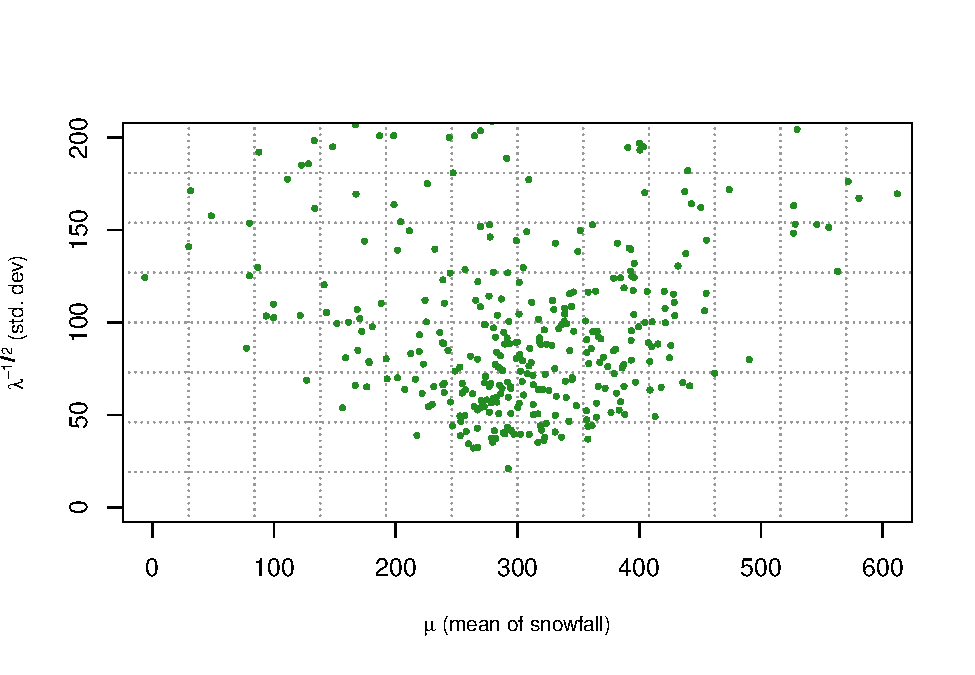
\includegraphics{note_stat561_files/figure-latex/unnamed-chunk-5-1}

\texttt{p.\ 9}

Let \(g(x_1,..,x_n)\) be a new random variable

\textbf{Definition}

\[E[g(\vec X)]=\begin{cases}\sum\cdots\sum_{all\vec x} g(\vec x)p(\vec x) \\ \idotsint_{\mathbf{R^n}}g(\vec x)f(\vec x)d\vec x\end{cases}\]

\[Eg(X,Y)=\int_{-\infty}^{\infty}\int_{-\infty}^{\infty} g(x, y)f(x, y) dx dy\].

\texttt{2018.11.27\textasciigrave{}\textasciigrave{}p.\ 10-11}

In our example, find \(E[X_1+X_2]\)

\begin{itemize}
\tightlist
\item
  Method 1
\end{itemize}

\[E[X_1+X_2]=\int_0^1\int_0^{x_2}(x_1+x_2)8x_1x_2dx_1dx_2=\int_0^1\int_0^{x_2}(8x_1^2x_2+8x_1x_2^2)dx_1dx_2=\int_0^1\left.(\frac{8x_1^3x_2}3+\frac{8x_1^2x_2^2}2)\right|_{x_1=0}^{x_2}dx_2\]

\[=\int_0^1(\frac{8x_2^4}3+\frac{8x_2^4}2)dx_2=\frac{20}3\int_0^1x_2^4dx_2=\frac{20}3\left.\frac{x_2^5}5\right|_0^1=\frac43\]

Method 2

\[E[X_1+X_2]=E[X_1]+E[X_2]=\int_0^1x_1(4x_1-4x_1^3)dx_1+\int_0^1x_24x_2^3dx_2=\frac8{15}+\frac45=\frac43\]

\texttt{2019.01.15\textasciigrave{}\textasciigrave{}p.1}

The joint probability dist ribu tion of (X, Y) can be completely
described with the \textbf{joint cdf (cumulative distr ib ution
function)} rather than with the joint pmf or jointpdf. The joint cdf is
the function \(F(x, y)\) defined by \[F(x,y) = P(X\le x, Y\le y)\] for
all \((x,y)\in\mathcal{R}\). The joint cdf is usually not very handy to
use for a discrete random vector. But for a continuous bivariate random
vector we have the important relationship , as in the univariate case,

\[F(x,y) =\int_{-\infty}^{y}\int_{-\infty}^{x}f(s,t)dsdt\]

From the bivariate Fundamental Theore m of Calcu lus, this implies that

\[\frac{\partial^2F(x,y)}{\partial x\partial y}=f(x,y)\]

at continuity points of \(f(x, y)\). This relationship is useful in sit
uations where an expression for \(F(x,y)\) can be found. The mixed
partial derivative can be computed to find the joint pdf.

\hypertarget{conditional-distributions-and-independence}{%
\subsection{4.2 Conditional Distributions and
Independence}\label{conditional-distributions-and-independence}}

\texttt{2018.11.27\textasciigrave{}\textasciigrave{}p.\ 12}

\[f(x_2|x_1)=\frac{f(x_1,x_2)}{f_1(x_1)};\quad p(x_2|x_1)=\frac{p(x_1,x_2)}{p_1(x_1)}\]

Note:

\[\int_{all\ x_2} f(x_2|x_1)dx_2=\int_{all\ x_2}\frac{f(x_1,x_2)}{f_1(x_1)}dx_2=\frac1{f_1(x_1)}\int_{all\ x_2}{f(x_1,x_2)}dx_2=1\]

\textbf{Definition 4.2.1} Let (X,Y) be a discrete bivariate random
vector with joint pmf f(x,y) and marginal pmfs \(f_X(x)\) and
\(f_Y(y)\). For any x such that \(P(X=x)=f_X(x)>0\), the conditional pmf
of Y given that \(X=x\) is the function of y denoted by \(f(y|x)\) are
defined by

\[f(y|x)=P(Y=y|X=x)=\frac{f(x,y)}{f_X(x)}\]

For any y such that \(P(Y=y)=f_Y(y)>0\), the conditional pmf of X given
that \(Y=y\) is the function of x denoted by \(f(x|y)\) are defined by

\[f(x|y)=P(X=x|Y=y)=\frac{f(x,y)}{f_Y(y)}\]

This function of y defines a pmf for a random variable. \(f(y|x)\ge0\)
for every y since \(f(x,y)\ge0\) and \(f_X(x)>0\). And

\[\sum_yf(y|x)=\frac{\sum_yf(x,y)}{f_X(x)}=\frac{f_X(x)}{f_X(x)}=1\]

\textbf{Definition 4.2.3} Let (X, Y) be a continuous bivariate random
vector with joint pdf f(x,y) and marginal pdfs f\_X(x) and f\_Y(y). For
any x such that \(f_X(x)>0\), the conditional pdf of Y given that
\(X=x\) is the function of y denoted by \(f(y|x)\) and defined by

\[f(y|x)=\frac{f(x,y)}{f_X(x)}\]

For any y such that \(f_Y(y)>0\), the conditional pdf of X given that
\(Y=y\) is the function of x denoted by \(f(x|y)\) and defined by

\[f(x|y)=\frac{f(x,y)}{f_Y(y)}\]

\texttt{2018.11.27\textasciigrave{}\textasciigrave{}p.\ 13}

Let \(g(x_2)\) be a function of \(X_2\)

\[E(g(x_2)|x_1)=\sum_{all\ x_2}g(x_2)p(x_2|x_1)\quad \text{and}\quad E(g(x_2)|x_1)=\int_{all\ x_2}g(x_2)f(x_2|x_1)dx_2\]

If g(Y) is a function of Y, then the conditional expected value of g(Y)
given that \(X=x\) is denoted by \(E(g(Y)|x)\) and is given by

\[E(g(Y)|x)=\sum_yg(y)f(y|x)\quad \text{and}\quad E(g(Y)|x)=\int_{-\infty}^{\infty}g(y)f(y|x)dy\]

\texttt{2018.11.27\textasciigrave{}\textasciigrave{}p.\ 14-16}

Example: \(f(x_1,x_2)=\frac12e^{-(x_1+x_2)}\), \(x_2>0,x_2>-2x_1\), find
\(f(x_2|x_1)\)

\[f_1(x_1)=\int_{all\ x_2}f(x_1,x_2)dx_2=\begin{cases}\int_0^{\infty}e^{-(x_1+x_2)}dx_2 & x_1\ge0 \\ \int_{-2x_1}^{\infty}e^{-(x_1+x_2)}dx_2 & x_1<0 \end{cases}\]

\[=\begin{cases}\frac12e^{-x_1}[{-e^{-x_2}}]_{x_2=0}^{\infty}=0-(-\frac12e^{-x_1})=\frac12e^{-x_1} & x_1\ge0 \\ \frac12e^{-x_1}[{-e^{-x_2}}]_{x_2=-2x_1}^{\infty}=0+\frac12e^{-x_1}e^{2x_1}=\frac12e^{x_1} & x_1<0 \end{cases}=\frac12e^{-|x_1|},\ -\infty<x_1<\infty\]

\[f(x_2|x_1)=\frac{f(x_1,x_2)}{f_1(x_1)}=\frac{\frac12e^{-(x_1+x_2)}}{\frac12e^{-|x_1|}}=e^{|x_1|-x_1-x_2},\quad x_2>0,x_2>-2x_1\]

\texttt{2018.11.29} \texttt{p.\ 1-2}

New example: \(f(x,y)=10xy^4\), \(0<x<1, 0<y<1\), find \(f(y|x)\)

\begin{Shaded}
\begin{Highlighting}[]
\KeywordTok{plot}\NormalTok{(}\ControlFlowTok{function}\NormalTok{(x) \{}
\NormalTok{    x}
\NormalTok{\}, }\DataTypeTok{from =} \FloatTok{-0.5}\NormalTok{, }\DataTypeTok{to =} \FloatTok{1.5}\NormalTok{, }\DataTypeTok{axes =} \OtherTok{FALSE}\NormalTok{, }\DataTypeTok{asp =} \DecValTok{1}\NormalTok{, }\DataTypeTok{xlab =} \StringTok{"x1"}\NormalTok{, }
    \DataTypeTok{ylab =} \StringTok{"x2"}\NormalTok{)}
\KeywordTok{axis}\NormalTok{(}\DecValTok{1}\NormalTok{, }\DataTypeTok{pos =} \DecValTok{0}\NormalTok{, }\DataTypeTok{xlab =} \StringTok{"x1"}\NormalTok{)}
\KeywordTok{axis}\NormalTok{(}\DecValTok{2}\NormalTok{, }\DataTypeTok{pos =} \DecValTok{0}\NormalTok{, }\DataTypeTok{ylab =} \StringTok{"x2"}\NormalTok{)}
\KeywordTok{polygon}\NormalTok{(}\DataTypeTok{x =} \KeywordTok{c}\NormalTok{(}\DecValTok{0}\NormalTok{, }\DecValTok{1}\NormalTok{, }\DecValTok{1}\NormalTok{, }\DecValTok{0}\NormalTok{), }\DataTypeTok{y =} \KeywordTok{c}\NormalTok{(}\DecValTok{0}\NormalTok{, }\DecValTok{0}\NormalTok{, }\DecValTok{1}\NormalTok{, }\DecValTok{1}\NormalTok{), }\DataTypeTok{density =} \DecValTok{10}\NormalTok{, }\DataTypeTok{angle =} \DecValTok{45}\NormalTok{)}
\end{Highlighting}
\end{Shaded}

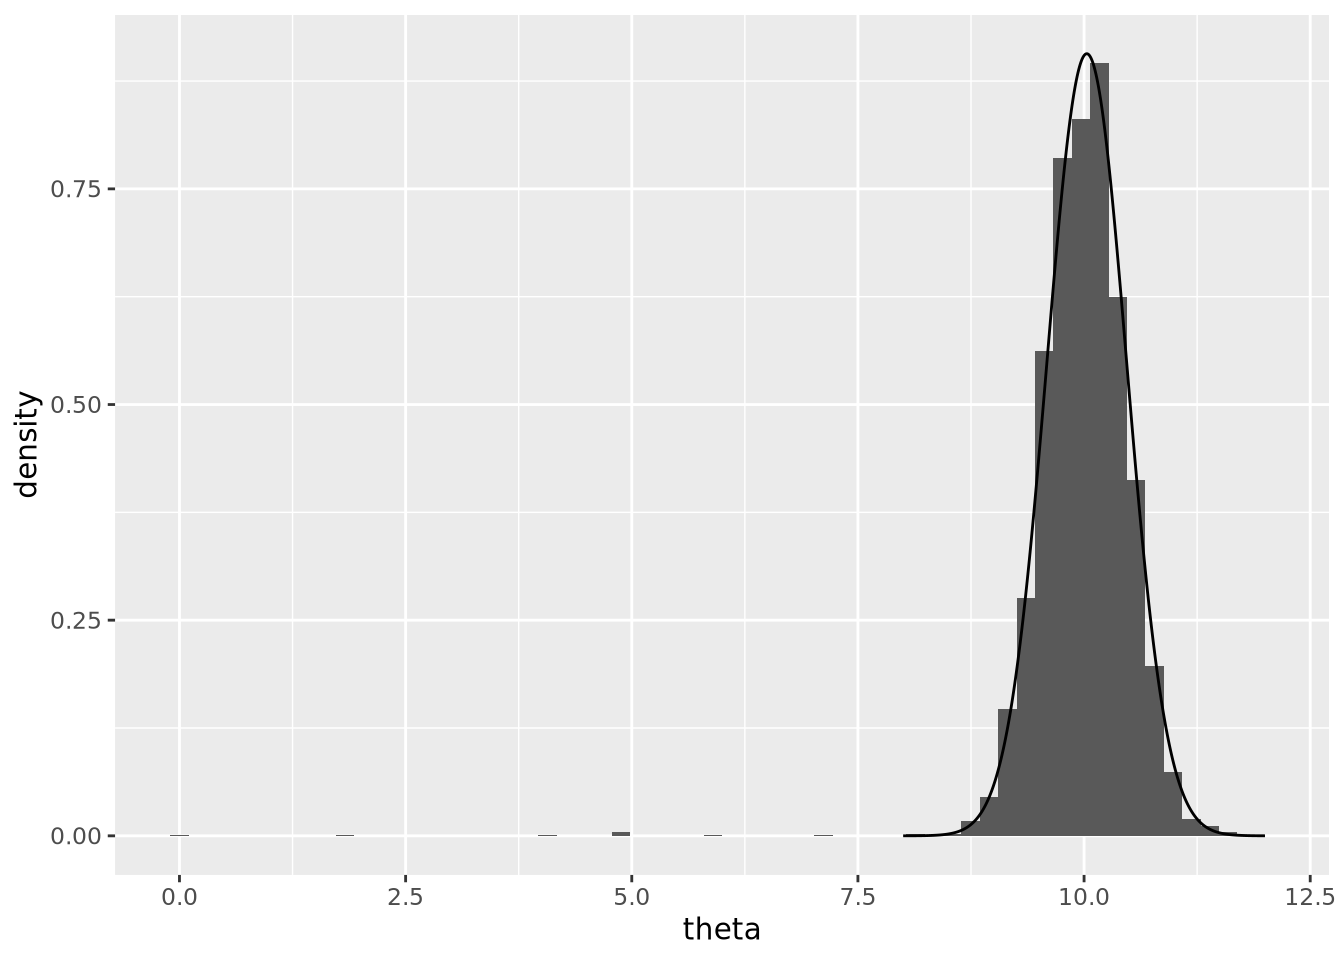
\includegraphics{note_stat561_files/figure-latex/unnamed-chunk-6-1}

Check

\[\int_0^1\int_0^110xy^4dxdy=\int_0^110y^4\left.\frac{x^2}2\right|_{x=0}^1dy=\int_0^110y^4\frac{1}2dy=5\left.\frac{y^5}5\right|_0^1=1\]

\[f_X(x)=\int_0^1f(x,y)dy=\int_0^110xy^4dy=10x\left.\frac{x^5}5\right|_0^1=2x,\quad0<x<1\]

\[f(y|x)=\frac{f(x,y)}{f_X(x)}=\frac{10xy^4}{2x}=5y^4,\quad 0<x<1,0<y<1\]

\textbf{Example 4.2.4 (Calculating conditional pdfs)}

The variance of the probability distribution described by \(f(y|x)\) is
called the conditional variance of Y given \(X=x\). Using the notation
\(Var(y|x)\) for this, we have, using the ordinary definition of
variance,

\[Var(y|x)=E(Y^2|x)-(E(Y|x))^2\]

\texttt{2019.1.8} \texttt{p.\ 1-2}

\[V[X|Y]=E[(X-E[X|Y])^2|Y]\]

\texttt{2018.11.29} \texttt{p.\ 3}

\textbf{Definition 4.2.5} Let (X,Y) be a bivariate random vector with
joint pdf or pmf f(x,y) and marginal pdfs or pmfs \(f_X(x)\) and
\(f_Y(y)\). Then X and Y are called \textbf{independent random variable}
if, for every \(x\in\mathbf{R}\) and \(y\in\mathbf{R}\),
\[f(x,y) = f_X(x)f_Y(y)\]

\textbf{Factorization Theorem}

\textbf{Lemma 4.2.7} Let (X,Y) be a bivariate random vector with joint
pdf or pmf f(x,y). X and Y are independent random variables if and only
if there exist functions g(x) and hey) such that, for every
\(x\in\mathbf{R}\) and \(y\in\mathbf{R}\),

\[f(x,y)=g(x)h(y)\]

\texttt{2018.11.29\textasciigrave{}\textasciigrave{}p.\ 4-6}

Proof: \(\Rightarrow\) trivial, based on difinition

\(\Leftarrow\): Suppose \(\exists\ g(x),h(y)\) such that
\(f(x,y)=g(x)h(y)\), then

\[f_X(x)=\int_{-\infty}^{\infty}f(x,y)dy=\int_{-\infty}^{\infty}g(x)h(y)dy=g(x)\int_{-\infty}^{\infty}h(y)dy\]

\(\int_{-\infty}^{\infty}h(y)dy=k\), Now \(f_X(x)=kg(x)\). Also

\[1=\int_{-\infty}^{\infty}f_X(x)dx=\int_{-\infty}^{\infty}kg(x)dx=k\int_{-\infty}^{\infty}g(x)dx,\quad \text{so } \int_{-\infty}^{\infty}g(x)dx=\frac1k\]

\[f_Y(y)=\int_{-\infty}^{\infty}f(x,y)dx=\int_{-\infty}^{\infty}g(x)h(y)dx=h(y)\int_{-\infty}^{\infty}g(x)dx=\frac1kh(y)\]

\[\therefore f(x,y)=g(x)h(y)=kg(x)\frac1kh(y)=f_X(x)f_Y(y)\]

So X and Y are independent.

\texttt{2018.11.29\textasciigrave{}\textasciigrave{}p.\ 7}

Example:

\begin{itemize}
\tightlist
\item
  Not independent
\end{itemize}

\[f(x,y)=c(x+y),\quad 0<x<1, 0<y<1\]

\[f(x,y)=cxy,\quad 0<x<y<1\quad =cxyI_{0<x<y<1}(x,y) \]

\begin{itemize}
\tightlist
\item
  Independent
\end{itemize}

\[f(x,y)=ce^{-(x+y)},\quad x>0, y>0\]

\texttt{2019.01.08} \texttt{p.\ 7-8}

\textbf{Theorem 4.2.10} Let X and Y be independent random variables.

\begin{enumerate}
\def\labelenumi{\alph{enumi}.}
\item
  For any \(A\subset\mathbf{R}\) and \(B\subset\mathbf{R}\),
  \(P(X\in A,Y\in B)=P(X\in A)P(Y\in B)\) that is, the events
  \{\(X\in A\)\} and \{\(Y\in B\)\} are independent events.
\item
  Let g(x) be a function only of x and h(y) be a function only of y.
  Then
\end{enumerate}

\[E(g(X)h(Y))=(Eg(X))(Eh(Y))\]

Proof:

\(E(g(X)h(Y))=\int_{-\infty}^{\infty}\int_{-\infty}^{\infty}g(x)h(y)f(x,y)dxdy=\int_{-\infty}^{\infty}h(y)f_Y(y)\left[\int_{-\infty}^{\infty}g(x)f_X(x)dx\right]dy=E[g(x)]E[h(y)]=(Eg(X))(Eh(Y))\)

In perticular, if X andY are independet, then \(E[XY]=E[X]E[Y]\)

\texttt{2019.01.08\textasciigrave{}\textasciigrave{}p.11}

\textbf{Theorem 4.2.12} Let X and Y be independent random variables with
moment generating functions \(M_X(t)\) and \(M_Y(t)\). Then the moment
generating function of the random variable \(Z=X+Y\) is given by

\[M_Z(t)=M_X(t)M_Y(t)\]

Proof:

\(M_W(t)=E[e^{tW}]=E[e^{t(X+Y)}]=E[e^{tX}+e^{tY}]=E[e^{tX}]+E[e^{tY}]=M_X(t)M_Y(t)\)

\textbf{Theorem 4.2.14} Let \(X\sim n(\mu,\sigma^2)\) and
\(Y\sim n(\gamma,\tau^2)\) be independent normal random variables, Then
the random variable \(Z=X+Y\) has a \(n(\mu+\gamma,\sigma^2+\tau^2)\)
distribution.



\end{document}
